\documentclass[twoside]{book}

% Packages required by doxygen
\usepackage{fixltx2e}
\usepackage{calc}
\usepackage{doxygen}
\usepackage[export]{adjustbox} % also loads graphicx
\usepackage{graphicx}
\usepackage[utf8]{inputenc}
\usepackage{makeidx}
\usepackage{multicol}
\usepackage{multirow}
\PassOptionsToPackage{warn}{textcomp}
\usepackage{textcomp}
\usepackage[nointegrals]{wasysym}
\usepackage[table]{xcolor}

% Font selection
\usepackage[T1]{fontenc}
\usepackage[scaled=.90]{helvet}
\usepackage{courier}
\usepackage{amssymb}
\usepackage{sectsty}
\renewcommand{\familydefault}{\sfdefault}
\allsectionsfont{%
  \fontseries{bc}\selectfont%
  \color{darkgray}%
}
\renewcommand{\DoxyLabelFont}{%
  \fontseries{bc}\selectfont%
  \color{darkgray}%
}
\newcommand{\+}{\discretionary{\mbox{\scriptsize$\hookleftarrow$}}{}{}}

% Page & text layout
\usepackage{geometry}
\geometry{%
  a4paper,%
  top=2.5cm,%
  bottom=2.5cm,%
  left=2.5cm,%
  right=2.5cm%
}
\tolerance=750
\hfuzz=15pt
\hbadness=750
\setlength{\emergencystretch}{15pt}
\setlength{\parindent}{0cm}
\setlength{\parskip}{3ex plus 2ex minus 2ex}
\makeatletter
\renewcommand{\paragraph}{%
  \@startsection{paragraph}{4}{0ex}{-1.0ex}{1.0ex}{%
    \normalfont\normalsize\bfseries\SS@parafont%
  }%
}
\renewcommand{\subparagraph}{%
  \@startsection{subparagraph}{5}{0ex}{-1.0ex}{1.0ex}{%
    \normalfont\normalsize\bfseries\SS@subparafont%
  }%
}
\makeatother

% Headers & footers
\usepackage{fancyhdr}
\pagestyle{fancyplain}
\fancyhead[LE]{\fancyplain{}{\bfseries\thepage}}
\fancyhead[CE]{\fancyplain{}{}}
\fancyhead[RE]{\fancyplain{}{\bfseries\leftmark}}
\fancyhead[LO]{\fancyplain{}{\bfseries\rightmark}}
\fancyhead[CO]{\fancyplain{}{}}
\fancyhead[RO]{\fancyplain{}{\bfseries\thepage}}
\fancyfoot[LE]{\fancyplain{}{}}
\fancyfoot[CE]{\fancyplain{}{}}
\fancyfoot[RE]{\fancyplain{}{\bfseries\scriptsize Generated by Doxygen }}
\fancyfoot[LO]{\fancyplain{}{\bfseries\scriptsize Generated by Doxygen }}
\fancyfoot[CO]{\fancyplain{}{}}
\fancyfoot[RO]{\fancyplain{}{}}
\renewcommand{\footrulewidth}{0.4pt}
\renewcommand{\chaptermark}[1]{%
  \markboth{#1}{}%
}
\renewcommand{\sectionmark}[1]{%
  \markright{\thesection\ #1}%
}

% Indices & bibliography
\usepackage{natbib}
\usepackage[titles]{tocloft}
\setcounter{tocdepth}{3}
\setcounter{secnumdepth}{5}
\makeindex

% Hyperlinks (required, but should be loaded last)
\usepackage{ifpdf}
\ifpdf
  \usepackage[pdftex,pagebackref=true]{hyperref}
\else
  \usepackage[ps2pdf,pagebackref=true]{hyperref}
\fi
\hypersetup{%
  colorlinks=true,%
  linkcolor=blue,%
  citecolor=blue,%
  unicode%
}

% Custom commands
\newcommand{\clearemptydoublepage}{%
  \newpage{\pagestyle{empty}\cleardoublepage}%
}

\usepackage{caption}
\captionsetup{labelsep=space,justification=centering,font={bf},singlelinecheck=off,skip=4pt,position=top}

%===== C O N T E N T S =====

\begin{document}

% Titlepage & ToC
\hypersetup{pageanchor=false,
             bookmarksnumbered=true,
             pdfencoding=unicode
            }
\pagenumbering{alph}
\begin{titlepage}
\vspace*{7cm}
\begin{center}%
{\Large Deoxygen\+Test }\\
\vspace*{1cm}
{\large Generated by Doxygen 1.8.14}\\
\end{center}
\end{titlepage}
\clearemptydoublepage
\pagenumbering{roman}
\tableofcontents
\clearemptydoublepage
\pagenumbering{arabic}
\hypersetup{pageanchor=true}

%--- Begin generated contents ---
\chapter{Robotic-\/\+Football-\/\+All-\/\+In-\/\+Many}
\label{md__r_e_a_d_m_e}
\Hypertarget{md__r_e_a_d_m_e}
This is the multi-\/file code for the robotic football team. The design philosophy behind this project is to divide the code amoung a number of classes file to make it easy to maintain and share code between robots. The abilities of the robot to be programmed are then chosen from a list of define statements in \mbox{\hyperlink{_config_8hpp_source}{config.\+hpp}}, like so\+:

In \mbox{\hyperlink{_config_8hpp_source}{config.\+hpp}}\+: 
\begin{DoxyCode}
\{c++\}
//#define BASIC\_DRIVETRAIN
#define OMNIWHEEL\_DRIVETRAIN
//#define CENTER\_PERIPHERALS
#define QB\_PERIPHERALS
//#define KICKER\_PERIPHERALS
//#define RECEIVER\_PERIPHERALS
#define LED\_STRIP
#define TACKLE
\end{DoxyCode}
 This example would create a robot that uses an omniwheel drivetrain (specifically our quarterback), with the led strip and tackle sensor enabled. At the end of the file are a list of error cases that the compile goes through to make sure no incompatable options are shown.

\subsection*{\#\#\#\# Useful Libraries }


\begin{DoxyEnumerate}
\item (P\+S3 Integration) \href{https://github.com/felis/USB_Host_Shield_2.0}{\tt U\+SB Host\+Shield 2.\+0}
\item (Omniwheel Rotation Locking) \href{https://github.com/adafruit/Adafruit_BNO055}{\tt Adafruit B\+N\+O055}
\item (S\+TL for arduino) \href{https://github.com/maniacbug/StandardCplusplus}{\tt Standard\+Cplusplus}
\end{DoxyEnumerate}

\subsection*{\#\#\#\# Controls }


\begin{DoxyItemize}
\item {\bfseries Basic Drivetrain}
\begin{DoxyItemize}
\item {\itshape Up/\+Down Left Joystick} -\/ Forward and Backward movement
\item {\itshape Left/\+Right Right Joystick} -\/ Turning
\item {\itshape R2} -\/ activates \char`\"{}boost\char`\"{}
\item {\itshape Start} -\/ Puts robot in \char`\"{}kids mode\char`\"{}. The speed is reduced, boost is disabled, and the leds will change
\item {\itshape Select \+\_\+-\/ Calibration mode -\/ disables drivetrain while changes are made
\begin{DoxyItemize}
\item \+\_\+\+Up/\+Down D-\/\+Pad -\/ compensates for drag left or right
\item {\itshape Select} -\/ exit Calibration Mode to regular drive mode
\end{DoxyItemize}}
\end{DoxyItemize}
\item {\itshape {\bfseries \mbox{\hyperlink{class_center}{Center}}}
\begin{DoxyItemize}
\item \mbox{\hyperlink{class_center}{Center}} currently uses basic drivetrain
\item {\itshape T\+R\+I\+A\+N\+G\+LE} -\/ raise the center release servo
\item {\itshape C\+R\+O\+SS} -\/ lower the center release servo
\end{DoxyItemize}}
\item {\itshape {\bfseries Omniwheel Drivetrain}
\begin{DoxyItemize}
\item {\itshape Up/\+Down/\+Left/\+Right Left Joystick} -\/ Lateral movement in any direction
\item {\itshape Up/\+Down/\+Left/\+Right D-\/\+Pad}-\/ Lateral Movement along compass directions at full power
\item {\itshape Left/\+Right Right Joystick} -\/ Turning -\/ as of version 1.\+0.\+3 this will disable rotation correction
\item {\itshape R3} (Right Joystick Press) -\/ Re-\/engage rotation correction
\item {\itshape R2} -\/ slow down speed
\item {\itshape L1} -\/ reverse directions (make back of robot front and vise versa)
\item Throwing
\begin{DoxyItemize}
\item {\itshape S\+Q\+U\+A\+RE} -\/ Handoff throw
\item {\itshape C\+R\+O\+SS} -\/ Reciever handoff throw/weak toss
\item {\itshape C\+I\+R\+C\+LE} -\/ mid range throw
\item {\itshape T\+R\+I\+A\+N\+G\+LE} -\/ max power throw
\item {\itshape R1} -\/ return thrower to down position
\item {\itshape L2} -\/ hold to enable throw offset
\begin{DoxyItemize}
\item {\itshape Up/\+Down D-\/\+Pad} -\/ adjust power of all throws but triangle
\end{DoxyItemize}
\end{DoxyItemize}
\end{DoxyItemize}}
\item {\itshape {\bfseries \mbox{\hyperlink{class_kicker}{Kicker}}}
\begin{DoxyItemize}
\item \mbox{\hyperlink{class_kicker}{Kicker}} -\/ currently uses basic drivetrain
\item {\itshape C\+R\+O\+SS} -\/ kick
\item {\itshape T\+R\+I\+A\+N\+G\+LE} -\/ reload 
\end{DoxyItemize}}
\end{DoxyItemize}
\chapter{Module Index}
\section{Modules}
Here is a list of all modules\+:\begin{DoxyCompactList}
\item \contentsline{section}{Peripherals}{\pageref{group___peripherals}}{}
\item \contentsline{section}{Robot}{\pageref{group___robot}}{}
\item \contentsline{section}{Containers}{\pageref{group___containers}}{}
\item \contentsline{section}{Drive\+Train}{\pageref{group___drive_train}}{}
\end{DoxyCompactList}

\chapter{Hierarchical Index}
\section{Class Hierarchy}
This inheritance list is sorted roughly, but not completely, alphabetically\+:\begin{DoxyCompactList}
\item \contentsline{section}{Valpo\+Robotics\+:\+:array$<$ T, S\+I\+ZE $>$}{\pageref{class_valpo_robotics_1_1array}}{}
\item \contentsline{section}{Valpo\+Robotics\+:\+:array$<$ Peripheral $\ast$, M\+A\+X\+\_\+\+T\+O\+T\+A\+L\+\_\+\+P\+E\+R\+I\+P\+E\+R\+A\+LS $>$}{\pageref{class_valpo_robotics_1_1array}}{}
\item \contentsline{section}{Drive\+Train}{\pageref{class_drive_train}}{}
\begin{DoxyCompactList}
\item \contentsline{section}{Basic\+Drive\+Controller}{\pageref{class_basic_drive_controller}}{}
\item \contentsline{section}{New\+Omni\+Drive}{\pageref{class_new_omni_drive}}{}
\item \contentsline{section}{Omni\+Drive\+Conrtoller}{\pageref{class_omni_drive_conrtoller}}{}
\item \contentsline{section}{test\+Drive\+Conrtoller}{\pageref{classtest_drive_conrtoller}}{}
\end{DoxyCompactList}
\item \contentsline{section}{L\+ED}{\pageref{class_l_e_d}}{}
\item \contentsline{section}{Motor}{\pageref{class_motor}}{}
\item \contentsline{section}{Peripheral}{\pageref{class_peripheral}}{}
\begin{DoxyCompactList}
\item \contentsline{section}{Center}{\pageref{class_center}}{}
\item \contentsline{section}{Drop\+Detector}{\pageref{class_drop_detector}}{}
\item \contentsline{section}{Empty\+Peripheral}{\pageref{class_empty_peripheral}}{}
\item \contentsline{section}{Kicker}{\pageref{class_kicker}}{}
\item \contentsline{section}{Peripheral\+Name}{\pageref{class_peripheral_name}}{}
\item \contentsline{section}{Q\+B\+Arm}{\pageref{class_q_b_arm}}{}
\item \contentsline{section}{Tackle\+Seansor}{\pageref{class_tackle_seansor}}{}
\end{DoxyCompactList}
\item \contentsline{section}{Robot}{\pageref{class_robot}}{}
\end{DoxyCompactList}

\chapter{Class Index}
\section{Class List}
Here are the classes, structs, unions and interfaces with brief descriptions\+:\begin{DoxyCompactList}
\item\contentsline{section}{\mbox{\hyperlink{class_valpo_robotics_1_1array}{Valpo\+Robotics\+::array$<$ T, S\+I\+Z\+E $>$}} \\*Container that allows each member to be accessed in a range based for loop }{\pageref{class_valpo_robotics_1_1array}}{}
\item\contentsline{section}{\mbox{\hyperlink{class_basic_drive_controller}{Basic\+Drive\+Controller}} \\*This is the basic drivetrain that most robots use Used for most two motor robots }{\pageref{class_basic_drive_controller}}{}
\item\contentsline{section}{\mbox{\hyperlink{class_center}{Center}} \\*This class controls the centers dropper arm this class controlls the dropper arm that drops the football on a snap }{\pageref{class_center}}{}
\item\contentsline{section}{\mbox{\hyperlink{class_drive_train}{Drive\+Train}} \\*This class is the parent class for all other drive trains }{\pageref{class_drive_train}}{}
\item\contentsline{section}{\mbox{\hyperlink{class_drop_detector}{Drop\+Detector}} }{\pageref{class_drop_detector}}{}
\item\contentsline{section}{\mbox{\hyperlink{class_empty_peripheral}{Empty\+Peripheral}} }{\pageref{class_empty_peripheral}}{}
\item\contentsline{section}{\mbox{\hyperlink{class_kicker}{Kicker}} \\*This class controls the kicker peripheral }{\pageref{class_kicker}}{}
\item\contentsline{section}{\mbox{\hyperlink{class_l_e_d}{L\+ED}} \\*This class controls the robots L\+E\+Ds }{\pageref{class_l_e_d}}{}
\item\contentsline{section}{\mbox{\hyperlink{class_motor}{Motor}} }{\pageref{class_motor}}{}
\item\contentsline{section}{\mbox{\hyperlink{class_new_omni_drive}{New\+Omni\+Drive}} }{\pageref{class_new_omni_drive}}{}
\item\contentsline{section}{\mbox{\hyperlink{class_omni_drive_conrtoller}{Omni\+Drive\+Conrtoller}} \\*This is the drive train for omniwheel robots Used for most four motor robots }{\pageref{class_omni_drive_conrtoller}}{}
\item\contentsline{section}{\mbox{\hyperlink{class_peripheral}{Peripheral}} \\*This class is the parent class for all other drive trains }{\pageref{class_peripheral}}{}
\item\contentsline{section}{\mbox{\hyperlink{class_peripheral_name}{Peripheral\+Name}} \\*Provide an example }{\pageref{class_peripheral_name}}{}
\item\contentsline{section}{\mbox{\hyperlink{class_q_b_arm}{Q\+B\+Arm}} \\*This class controls the quaterback\textquotesingle{}s arm }{\pageref{class_q_b_arm}}{}
\item\contentsline{section}{\mbox{\hyperlink{class_robot}{Robot}} \\*Class that acts as a wrapper for other classes }{\pageref{class_robot}}{}
\item\contentsline{section}{\mbox{\hyperlink{class_tackle_seansor}{Tackle\+Seansor}} \\*This class controls the tackle sensor and its interaction with the L\+E\+Ds }{\pageref{class_tackle_seansor}}{}
\item\contentsline{section}{\mbox{\hyperlink{classtest_drive_conrtoller}{test\+Drive\+Conrtoller}} }{\pageref{classtest_drive_conrtoller}}{}
\end{DoxyCompactList}

\chapter{Module Documentation}
\hypertarget{group___peripherals}{}\section{Peripherals}
\label{group___peripherals}\index{Peripherals@{Peripherals}}

\hypertarget{group___robot}{}\section{Robot}
\label{group___robot}\index{Robot@{Robot}}
\subsection*{Classes}
\begin{DoxyCompactItemize}
\item 
class \mbox{\hyperlink{class_robot}{Robot}}
\begin{DoxyCompactList}\small\item\em Class that acts as a wrapper for other classes. \end{DoxyCompactList}\end{DoxyCompactItemize}


\subsection{Detailed Description}

\hypertarget{group___containers}{}\section{Containers}
\label{group___containers}\index{Containers@{Containers}}
\subsection*{Classes}
\begin{DoxyCompactItemize}
\item 
class \mbox{\hyperlink{class_valpo_robotics_1_1array}{Valpo\+Robotics\+::array$<$ T, S\+I\+Z\+E $>$}}
\begin{DoxyCompactList}\small\item\em container that allows each member to be accessed in a range based for loop \end{DoxyCompactList}\end{DoxyCompactItemize}


\subsection{Detailed Description}

\hypertarget{group___drive_train}{}\section{Drive\+Train}
\label{group___drive_train}\index{Drive\+Train@{Drive\+Train}}
\subsection*{Classes}
\begin{DoxyCompactItemize}
\item 
class \mbox{\hyperlink{class_basic_drive_controller}{Basic\+Drive\+Controller}}
\begin{DoxyCompactList}\small\item\em This is the basic drivetrain that most robots use Used for most two motor robots. \end{DoxyCompactList}\item 
class \mbox{\hyperlink{class_drive_train}{Drive\+Train}}
\begin{DoxyCompactList}\small\item\em This class is the parent class for all other drive trains. \end{DoxyCompactList}\item 
class \mbox{\hyperlink{class_omni_drive_conrtoller}{Omni\+Drive\+Conrtoller}}
\begin{DoxyCompactList}\small\item\em This is the drive train for omniwheel robots Used for most four motor robots. \end{DoxyCompactList}\end{DoxyCompactItemize}


\subsection{Detailed Description}

\chapter{Class Documentation}
\hypertarget{class_valpo_robotics_1_1array}{}\section{Valpo\+Robotics\+:\+:array$<$ T, S\+I\+ZE $>$ Class Template Reference}
\label{class_valpo_robotics_1_1array}\index{Valpo\+Robotics\+::array$<$ T, S\+I\+Z\+E $>$@{Valpo\+Robotics\+::array$<$ T, S\+I\+Z\+E $>$}}


container that allows each member to be accessed in a range based for loop  




{\ttfamily \#include $<$array.\+hpp$>$}

\subsection*{Public Member Functions}
\begin{DoxyCompactItemize}
\item 
\mbox{\Hypertarget{class_valpo_robotics_1_1array_ad1673d960bb1108221b2e5cb71dc1134}\label{class_valpo_robotics_1_1array_ad1673d960bb1108221b2e5cb71dc1134}} 
T $\ast$ \mbox{\hyperlink{class_valpo_robotics_1_1array_ad1673d960bb1108221b2e5cb71dc1134}{begin}} ()
\begin{DoxyCompactList}\small\item\em function that returns p\+Begin implemented so range based for loop will work \end{DoxyCompactList}\item 
\mbox{\Hypertarget{class_valpo_robotics_1_1array_a8b00881ddaed31c468e80020b275fe40}\label{class_valpo_robotics_1_1array_a8b00881ddaed31c468e80020b275fe40}} 
T $\ast$ \mbox{\hyperlink{class_valpo_robotics_1_1array_a8b00881ddaed31c468e80020b275fe40}{end}} ()
\begin{DoxyCompactList}\small\item\em function that returns p\+End implemented so range based for loop will work \end{DoxyCompactList}\item 
\mbox{\Hypertarget{class_valpo_robotics_1_1array_ab0d7f3c67b7928bd11b0fab2e5970d55}\label{class_valpo_robotics_1_1array_ab0d7f3c67b7928bd11b0fab2e5970d55}} 
void \mbox{\hyperlink{class_valpo_robotics_1_1array_ab0d7f3c67b7928bd11b0fab2e5970d55}{push\+\_\+back}} (T next\+Element)
\begin{DoxyCompactList}\small\item\em places an element in the next avaliable position if avaliable \end{DoxyCompactList}\end{DoxyCompactItemize}
\subsection*{Public Attributes}
\begin{DoxyCompactItemize}
\item 
\mbox{\Hypertarget{class_valpo_robotics_1_1array_a7769453fad25835d0cf35f577bc62faa}\label{class_valpo_robotics_1_1array_a7769453fad25835d0cf35f577bc62faa}} 
T \mbox{\hyperlink{class_valpo_robotics_1_1array_a7769453fad25835d0cf35f577bc62faa}{arr}} \mbox{[}S\+I\+ZE\mbox{]}
\begin{DoxyCompactList}\small\item\em underlying array \end{DoxyCompactList}\item 
\mbox{\Hypertarget{class_valpo_robotics_1_1array_a31464f62e42309a1ef2476910cade587}\label{class_valpo_robotics_1_1array_a31464f62e42309a1ef2476910cade587}} 
T $\ast$ \mbox{\hyperlink{class_valpo_robotics_1_1array_a31464f62e42309a1ef2476910cade587}{p\+Begin}} = \&(\mbox{\hyperlink{class_valpo_robotics_1_1array_a7769453fad25835d0cf35f577bc62faa}{arr}}\mbox{[}0\mbox{]})
\begin{DoxyCompactList}\small\item\em pointer to the start of the array \end{DoxyCompactList}\item 
\mbox{\Hypertarget{class_valpo_robotics_1_1array_a63deade950411259aa7a55a80b672cdf}\label{class_valpo_robotics_1_1array_a63deade950411259aa7a55a80b672cdf}} 
T $\ast$ \mbox{\hyperlink{class_valpo_robotics_1_1array_a63deade950411259aa7a55a80b672cdf}{p\+End}} = \mbox{\hyperlink{class_valpo_robotics_1_1array_a31464f62e42309a1ef2476910cade587}{p\+Begin}}
\begin{DoxyCompactList}\small\item\em pointer to the nex unused avaliable position in the array \end{DoxyCompactList}\end{DoxyCompactItemize}


\subsection{Detailed Description}
\subsubsection*{template$<$typename T, int S\+I\+ZE$>$\newline
class Valpo\+Robotics\+::array$<$ T, S\+I\+Z\+E $>$}

container that allows each member to be accessed in a range based for loop 

This container exists because std\+::array is unavaliable under arduino for no apparent reason. Do not use this in a non arduino context, use boost\+::array or std\+::array

\begin{DoxyNote}{Note}
Do not use this in a non arduino context.
\end{DoxyNote}
\begin{DoxyAuthor}{Author}
Bill Sullivan
\end{DoxyAuthor}
\begin{DoxyVersion}{Version}
\$\+Revision\+: 1.\+0
\end{DoxyVersion}
\begin{DoxyDate}{Date}
2018/08/14 14\+:16\+:20
\end{DoxyDate}
Created on\+: 2018/04/14 14\+:16\+:20 

The documentation for this class was generated from the following file\+:\begin{DoxyCompactItemize}
\item 
array.\+hpp\end{DoxyCompactItemize}

\hypertarget{class_basic_drive_controller}{}\section{Basic\+Drive\+Controller Class Reference}
\label{class_basic_drive_controller}\index{Basic\+Drive\+Controller@{Basic\+Drive\+Controller}}


This is the basic drivetrain that most robots use Used for most two motor robots.  




{\ttfamily \#include $<$Basic\+Drive.\+hpp$>$}

Inheritance diagram for Basic\+Drive\+Controller\+:\begin{figure}[H]
\begin{center}
\leavevmode
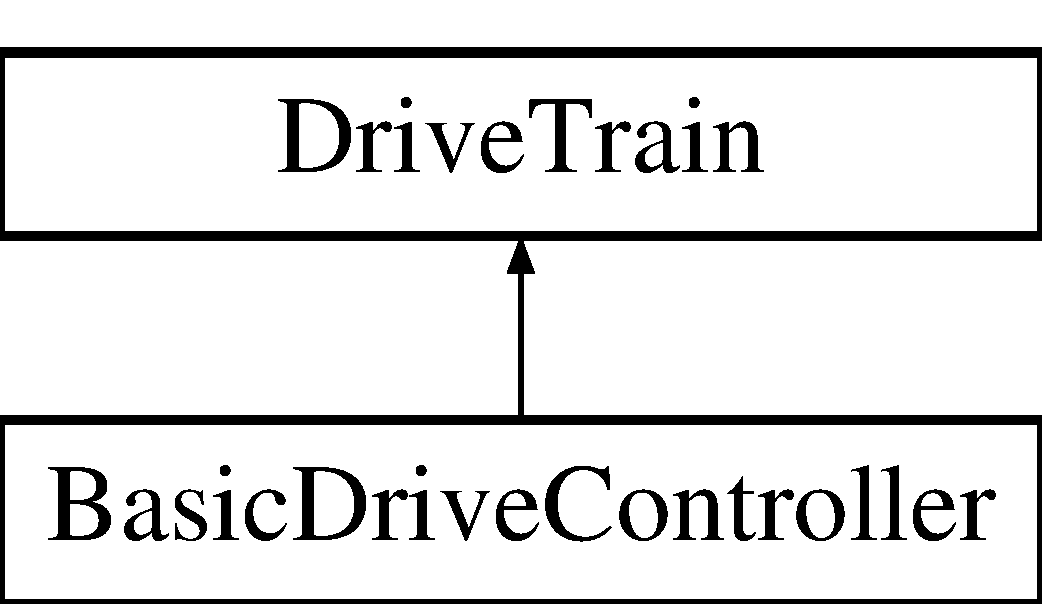
\includegraphics[height=2.000000cm]{class_basic_drive_controller}
\end{center}
\end{figure}
\subsection*{Public Member Functions}
\begin{DoxyCompactItemize}
\item 
\mbox{\Hypertarget{class_basic_drive_controller_a460f99786b7e701d72a91466f5cc8041}\label{class_basic_drive_controller_a460f99786b7e701d72a91466f5cc8041}} 
void \mbox{\hyperlink{class_basic_drive_controller_a460f99786b7e701d72a91466f5cc8041}{e\+Stop}} ()
\begin{DoxyCompactList}\small\item\em stop the robot so in the event control is lost controls what happens when the controller disconnects Make sure this code results in the robot stopping or we will break anouther door \end{DoxyCompactList}\item 
\mbox{\Hypertarget{class_basic_drive_controller_a11b639d12205bb597f07206df6721950}\label{class_basic_drive_controller_a11b639d12205bb597f07206df6721950}} 
void \mbox{\hyperlink{class_basic_drive_controller_a11b639d12205bb597f07206df6721950}{do\+Thing}} ()
\begin{DoxyCompactList}\small\item\em do\+Thing controls the calls functions that handel inputs and control motors calls functions that handel inputs and places those inputs into variables to be used later Then selects which control mode to use based on user input then calls a drivetrain funcion \end{DoxyCompactList}\item 
\mbox{\Hypertarget{class_basic_drive_controller_a511911167940331dcf369aaf925e9fde}\label{class_basic_drive_controller_a511911167940331dcf369aaf925e9fde}} 
void \mbox{\hyperlink{class_basic_drive_controller_a511911167940331dcf369aaf925e9fde}{setup}} ()
\begin{DoxyCompactList}\small\item\em sets initial values of variables and motors \end{DoxyCompactList}\end{DoxyCompactItemize}
\subsection*{Public Attributes}
\begin{DoxyCompactItemize}
\item 
\mbox{\Hypertarget{class_basic_drive_controller_a445c2c05f8d0096c27a8778f55735cec}\label{class_basic_drive_controller_a445c2c05f8d0096c27a8778f55735cec}} 
\mbox{\hyperlink{class_motor}{Motor}} \mbox{\hyperlink{class_basic_drive_controller_a445c2c05f8d0096c27a8778f55735cec}{left\+Motor}}
\begin{DoxyCompactList}\small\item\em Victors are modeled as Motors. \end{DoxyCompactList}\item 
\mbox{\Hypertarget{class_basic_drive_controller_aa7a52433c7991724f24d317fae6805a9}\label{class_basic_drive_controller_aa7a52433c7991724f24d317fae6805a9}} 
\mbox{\hyperlink{class_motor}{Motor}} {\bfseries right\+Motor}
\end{DoxyCompactItemize}
\subsection*{Protected Member Functions}
\begin{DoxyCompactItemize}
\item 
\mbox{\Hypertarget{class_basic_drive_controller_ae934462a6e905bd1660cdf6c307d779e}\label{class_basic_drive_controller_ae934462a6e905bd1660cdf6c307d779e}} 
const void \mbox{\hyperlink{class_basic_drive_controller_ae934462a6e905bd1660cdf6c307d779e}{arcade\+Drive}} ()
\begin{DoxyCompactList}\small\item\em function that controls how the robot controls under arcade controls \end{DoxyCompactList}\item 
\mbox{\Hypertarget{class_basic_drive_controller_ac454ab3b1872cc84138f29c4574680ef}\label{class_basic_drive_controller_ac454ab3b1872cc84138f29c4574680ef}} 
const void \mbox{\hyperlink{class_basic_drive_controller_ac454ab3b1872cc84138f29c4574680ef}{tank\+Drive}} ()
\begin{DoxyCompactList}\small\item\em function that controls how the robot controls under tank controls \end{DoxyCompactList}\item 
\mbox{\Hypertarget{class_basic_drive_controller_a6c5c51282655efdf990d6d01f7a36449}\label{class_basic_drive_controller_a6c5c51282655efdf990d6d01f7a36449}} 
void \mbox{\hyperlink{class_basic_drive_controller_a6c5c51282655efdf990d6d01f7a36449}{handel\+Inputs}} ()
\begin{DoxyCompactList}\small\item\em function that handels inputs \end{DoxyCompactList}\item 
\mbox{\Hypertarget{class_basic_drive_controller_a02d070214ca3ae4153b36d46b4b71318}\label{class_basic_drive_controller_a02d070214ca3ae4153b36d46b4b71318}} 
void \mbox{\hyperlink{class_basic_drive_controller_a02d070214ca3ae4153b36d46b4b71318}{invert\+Inputs}} ()
\begin{DoxyCompactList}\small\item\em invert inputs if inverting is true \end{DoxyCompactList}\end{DoxyCompactItemize}
\subsection*{Protected Attributes}
\begin{DoxyCompactItemize}
\item 
\mbox{\Hypertarget{class_basic_drive_controller_a5ad8d9c49caf2e2e373e4ba61502e3a3}\label{class_basic_drive_controller_a5ad8d9c49caf2e2e373e4ba61502e3a3}} 
int \mbox{\hyperlink{class_basic_drive_controller_a5ad8d9c49caf2e2e373e4ba61502e3a3}{drive\+Ctrl}}
\begin{DoxyCompactList}\small\item\em Flag that selects weather the robot is using Tank or Arcade control. \end{DoxyCompactList}\item 
\mbox{\Hypertarget{class_basic_drive_controller_af07886b0094095fdbc490df4d06b0e33}\label{class_basic_drive_controller_af07886b0094095fdbc490df4d06b0e33}} 
uint8\+\_\+t \mbox{\hyperlink{class_basic_drive_controller_af07886b0094095fdbc490df4d06b0e33}{state}}
\begin{DoxyCompactList}\small\item\em Flag that selects weather the robot is using kid or normal handcap Enter/\+Exit Kids mode by pressing start Kids mode makes the robot move slowly enough that it is safe to let a two year old drive it with minimal supervision. \end{DoxyCompactList}\item 
\mbox{\Hypertarget{class_basic_drive_controller_a5ea443561f5c7f79d86264a8fa9f107f}\label{class_basic_drive_controller_a5ea443561f5c7f79d86264a8fa9f107f}} 
int \mbox{\hyperlink{class_basic_drive_controller_a5ea443561f5c7f79d86264a8fa9f107f}{motor\+Correct}}
\begin{DoxyCompactList}\small\item\em variable that corrects for diffrences between each motor (Mostly irrlevent since bainbots moters were replaced) \end{DoxyCompactList}\item 
\mbox{\Hypertarget{class_basic_drive_controller_ae7b248880cef70b4e97037d9c0dcc00c}\label{class_basic_drive_controller_ae7b248880cef70b4e97037d9c0dcc00c}} 
uint8\+\_\+t \mbox{\hyperlink{class_basic_drive_controller_ae7b248880cef70b4e97037d9c0dcc00c}{inverting}}
\begin{DoxyCompactList}\small\item\em variable that selects if robot is driving backwords \end{DoxyCompactList}\item 
\mbox{\Hypertarget{class_basic_drive_controller_af011f366ab009c2567c516575926b281}\label{class_basic_drive_controller_af011f366ab009c2567c516575926b281}} 
uint8\+\_\+t \mbox{\hyperlink{class_basic_drive_controller_af011f366ab009c2567c516575926b281}{handicap}}
\begin{DoxyCompactList}\small\item\em motor power is divided by this variable \end{DoxyCompactList}\item 
\mbox{\Hypertarget{class_basic_drive_controller_a38c5c5e01542b9496643d54a6b1d489b}\label{class_basic_drive_controller_a38c5c5e01542b9496643d54a6b1d489b}} 
int \mbox{\hyperlink{class_basic_drive_controller_a38c5c5e01542b9496643d54a6b1d489b}{right\+InputY}}
\begin{DoxyCompactList}\small\item\em right stick\textquotesingle{}s up/down input \end{DoxyCompactList}\item 
\mbox{\Hypertarget{class_basic_drive_controller_a4506e85e8e9ae30629838b0bde6f14c6}\label{class_basic_drive_controller_a4506e85e8e9ae30629838b0bde6f14c6}} 
int \mbox{\hyperlink{class_basic_drive_controller_a4506e85e8e9ae30629838b0bde6f14c6}{left\+InputY}}
\begin{DoxyCompactList}\small\item\em left stick\textquotesingle{}s up/down input \end{DoxyCompactList}\item 
\mbox{\Hypertarget{class_basic_drive_controller_a82a214d753ed348d9cea96fa5e23fb8b}\label{class_basic_drive_controller_a82a214d753ed348d9cea96fa5e23fb8b}} 
int \mbox{\hyperlink{class_basic_drive_controller_a82a214d753ed348d9cea96fa5e23fb8b}{right\+InputX}}
\begin{DoxyCompactList}\small\item\em right stick\textquotesingle{}s left/right input \end{DoxyCompactList}\end{DoxyCompactItemize}


\subsection{Detailed Description}
This is the basic drivetrain that most robots use Used for most two motor robots. 

\begin{DoxyAuthor}{Author}
Bill Sullivan
\end{DoxyAuthor}
\begin{DoxyVersion}{Version}
\$\+Revision\+: 1.\+0
\end{DoxyVersion}
\begin{DoxyDate}{Date}
2018/08/15 14\+:16\+:20
\end{DoxyDate}
Created on\+: 2018/04/14 14\+:16\+:20 

The documentation for this class was generated from the following files\+:\begin{DoxyCompactItemize}
\item 
Drive\+Train/\+Basic\+Drive/Basic\+Drive.\+hpp\item 
Drive\+Train/\+Basic\+Drive/Basic\+Drive.\+cpp\end{DoxyCompactItemize}

\hypertarget{class_center}{}\section{Center Class Reference}
\label{class_center}\index{Center@{Center}}


This class controls the centers dropper arm this class controlls the dropper arm that drops the football on a snap.  




{\ttfamily \#include $<$center.\+hpp$>$}

Inheritance diagram for Center\+:\begin{figure}[H]
\begin{center}
\leavevmode
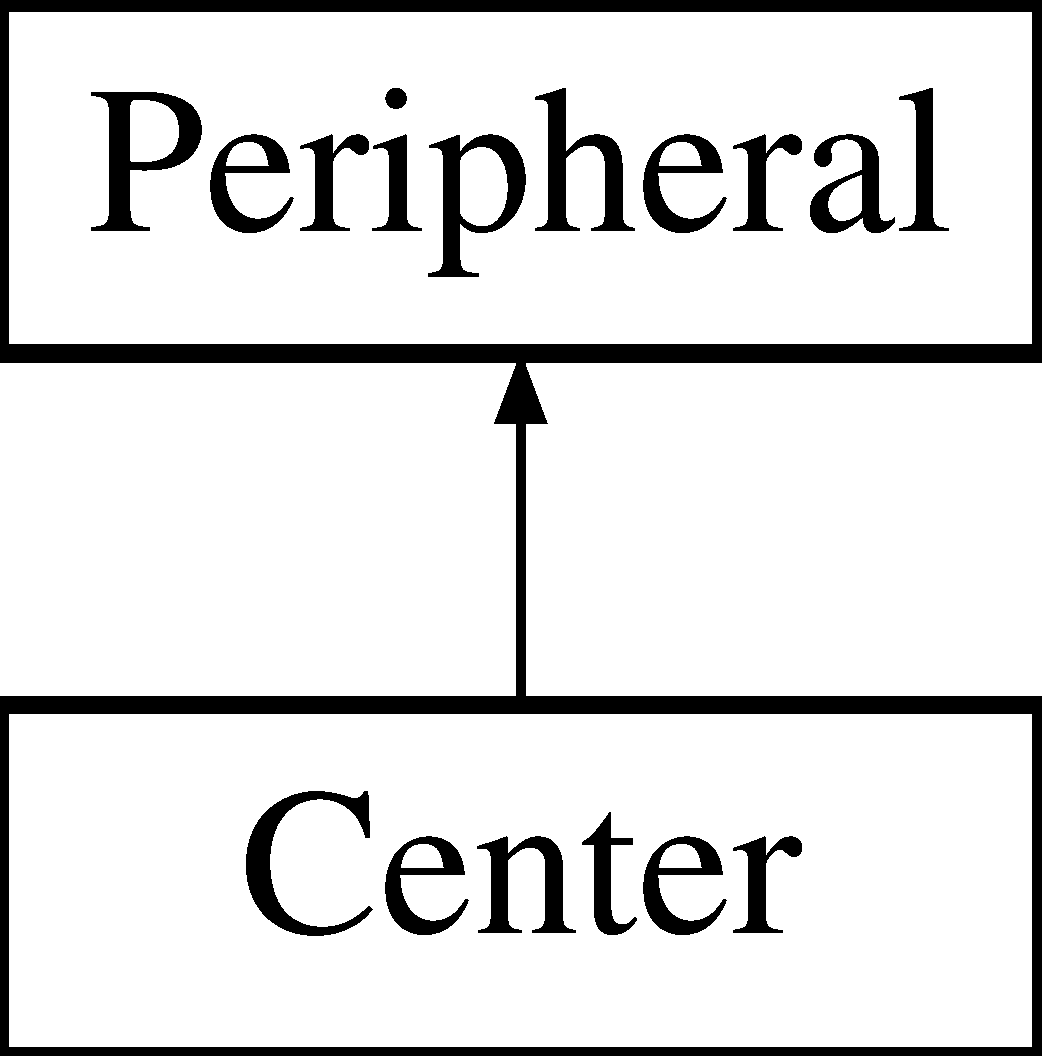
\includegraphics[height=2.000000cm]{class_center}
\end{center}
\end{figure}
\subsection*{Public Member Functions}
\begin{DoxyCompactItemize}
\item 
\mbox{\Hypertarget{class_center_a0fe884e8c678da837a4e6082ff344161}\label{class_center_a0fe884e8c678da837a4e6082ff344161}} 
void \mbox{\hyperlink{class_center_a0fe884e8c678da837a4e6082ff344161}{do\+Not\+Connected\+Thing}} ()
\begin{DoxyCompactList}\small\item\em ensure the robot enters a safe state when connection to the controller is lost \end{DoxyCompactList}\item 
\mbox{\Hypertarget{class_center_aa5fc180da844ce0bb60f163f1a819640}\label{class_center_aa5fc180da844ce0bb60f163f1a819640}} 
void \mbox{\hyperlink{class_center_aa5fc180da844ce0bb60f163f1a819640}{do\+Thing}} ()
\begin{DoxyCompactList}\small\item\em the implementation of do\+Thing should implement what happens when the controller is connected \end{DoxyCompactList}\item 
\mbox{\Hypertarget{class_center_a0b3dfd6c02ca9e0331db19fbaa026626}\label{class_center_a0b3dfd6c02ca9e0331db19fbaa026626}} 
void \mbox{\hyperlink{class_center_a0b3dfd6c02ca9e0331db19fbaa026626}{setup}} ()
\begin{DoxyCompactList}\small\item\em sets initial values of variables \end{DoxyCompactList}\end{DoxyCompactItemize}


\subsection{Detailed Description}
This class controls the centers dropper arm this class controlls the dropper arm that drops the football on a snap. 

\begin{DoxyAuthor}{Author}
Bill Sullivan
\end{DoxyAuthor}
\begin{DoxyVersion}{Version}
\$\+Revision\+: 1.\+0
\end{DoxyVersion}
\begin{DoxyDate}{Date}
2018/08/15 14\+:16\+:20
\end{DoxyDate}
Created on\+: 2018/04/14 14\+:16\+:20 

The documentation for this class was generated from the following files\+:\begin{DoxyCompactItemize}
\item 
Robotic\+Football\+Peripherals/\+Center\+Dropper/center.\+hpp\item 
Robotic\+Football\+Peripherals/\+Center\+Dropper/center.\+cpp\end{DoxyCompactItemize}

\hypertarget{class_drive_train}{}\section{Drive\+Train Class Reference}
\label{class_drive_train}\index{Drive\+Train@{Drive\+Train}}


This class is the parent class for all other drive trains.  




{\ttfamily \#include $<$Drive\+Train.\+hpp$>$}

Inheritance diagram for Drive\+Train\+:\begin{figure}[H]
\begin{center}
\leavevmode
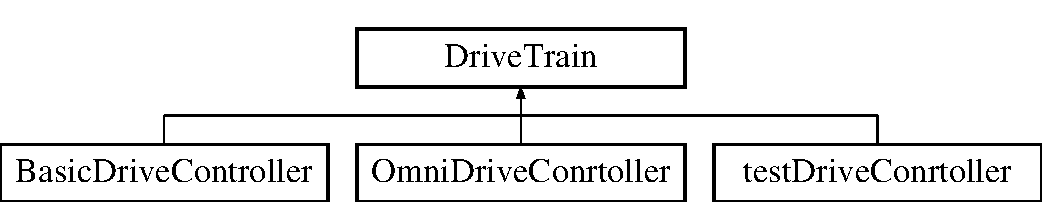
\includegraphics[height=2.000000cm]{class_drive_train}
\end{center}
\end{figure}
\subsection*{Public Member Functions}
\begin{DoxyCompactItemize}
\item 
\mbox{\Hypertarget{class_drive_train_ab56f1f7c0f20792e999ef85c374fc2dd}\label{class_drive_train_ab56f1f7c0f20792e999ef85c374fc2dd}} 
virtual void \mbox{\hyperlink{class_drive_train_ab56f1f7c0f20792e999ef85c374fc2dd}{e\+Stop}} ()
\begin{DoxyCompactList}\small\item\em the implementation of e\+Stop should implement what happens when the controller disconnects Make sure this code results in the robot stopping or we will break anouther door \end{DoxyCompactList}\item 
\mbox{\Hypertarget{class_drive_train_a3bfe7aec9ea012b074df4cd6e76d0a03}\label{class_drive_train_a3bfe7aec9ea012b074df4cd6e76d0a03}} 
virtual void \mbox{\hyperlink{class_drive_train_a3bfe7aec9ea012b074df4cd6e76d0a03}{do\+Thing}} ()
\begin{DoxyCompactList}\small\item\em the implementation of do\+Thing should implement what happens when the controller is connected \end{DoxyCompactList}\item 
\mbox{\Hypertarget{class_drive_train_aa931301c0de26dddf04236dd539ab1df}\label{class_drive_train_aa931301c0de26dddf04236dd539ab1df}} 
virtual void \mbox{\hyperlink{class_drive_train_aa931301c0de26dddf04236dd539ab1df}{setup}} ()
\begin{DoxyCompactList}\small\item\em the implementation of setup should implement setup code \end{DoxyCompactList}\end{DoxyCompactItemize}


\subsection{Detailed Description}
This class is the parent class for all other drive trains. 

This class is the parent class for all other drive trains

The only way this class should be used is as a parent class for other classes

\begin{DoxyNote}{Note}
Attempts at zen rarely work.
\end{DoxyNote}
\begin{DoxyAuthor}{Author}
Bill Sullivan
\end{DoxyAuthor}
\begin{DoxyVersion}{Version}
\$\+Revision\+: 1.\+0
\end{DoxyVersion}
\begin{DoxyDate}{Date}
2018/08/15 14\+:16\+:20
\end{DoxyDate}
Created on\+: 2018/04/14 14\+:16\+:20 

The documentation for this class was generated from the following file\+:\begin{DoxyCompactItemize}
\item 
Drive\+Train/Drive\+Train.\+hpp\end{DoxyCompactItemize}

\hypertarget{class_empty_peripheral}{}\section{Empty\+Peripheral Class Reference}
\label{class_empty_peripheral}\index{Empty\+Peripheral@{Empty\+Peripheral}}
Inheritance diagram for Empty\+Peripheral\+:\begin{figure}[H]
\begin{center}
\leavevmode
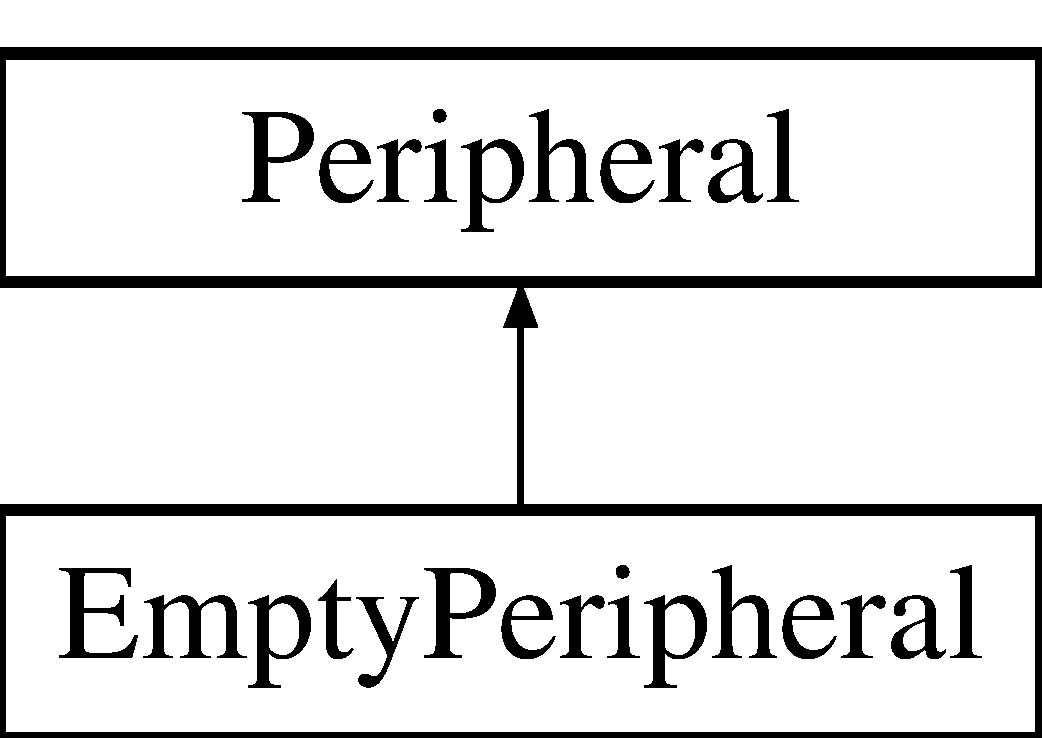
\includegraphics[height=2.000000cm]{class_empty_peripheral}
\end{center}
\end{figure}
\subsection*{Public Member Functions}
\begin{DoxyCompactItemize}
\item 
\mbox{\Hypertarget{class_empty_peripheral_a563da11bcb1e8b63a6472af037d1b38c}\label{class_empty_peripheral_a563da11bcb1e8b63a6472af037d1b38c}} 
void {\bfseries do\+Thing} ()
\item 
\mbox{\Hypertarget{class_empty_peripheral_a9a3476c5016dd2865fcad3bd76010069}\label{class_empty_peripheral_a9a3476c5016dd2865fcad3bd76010069}} 
void {\bfseries do\+Not\+Connected\+Thing} ()
\end{DoxyCompactItemize}


The documentation for this class was generated from the following file\+:\begin{DoxyCompactItemize}
\item 
Robotic\+Football\+Peripherals/Empty\+Peripheral.\+hpp\end{DoxyCompactItemize}

\hypertarget{class_kicker}{}\section{Kicker Class Reference}
\label{class_kicker}\index{Kicker@{Kicker}}


This class controls the kicker peripheral.  




{\ttfamily \#include $<$kicker.\+hpp$>$}

Inheritance diagram for Kicker\+:\begin{figure}[H]
\begin{center}
\leavevmode
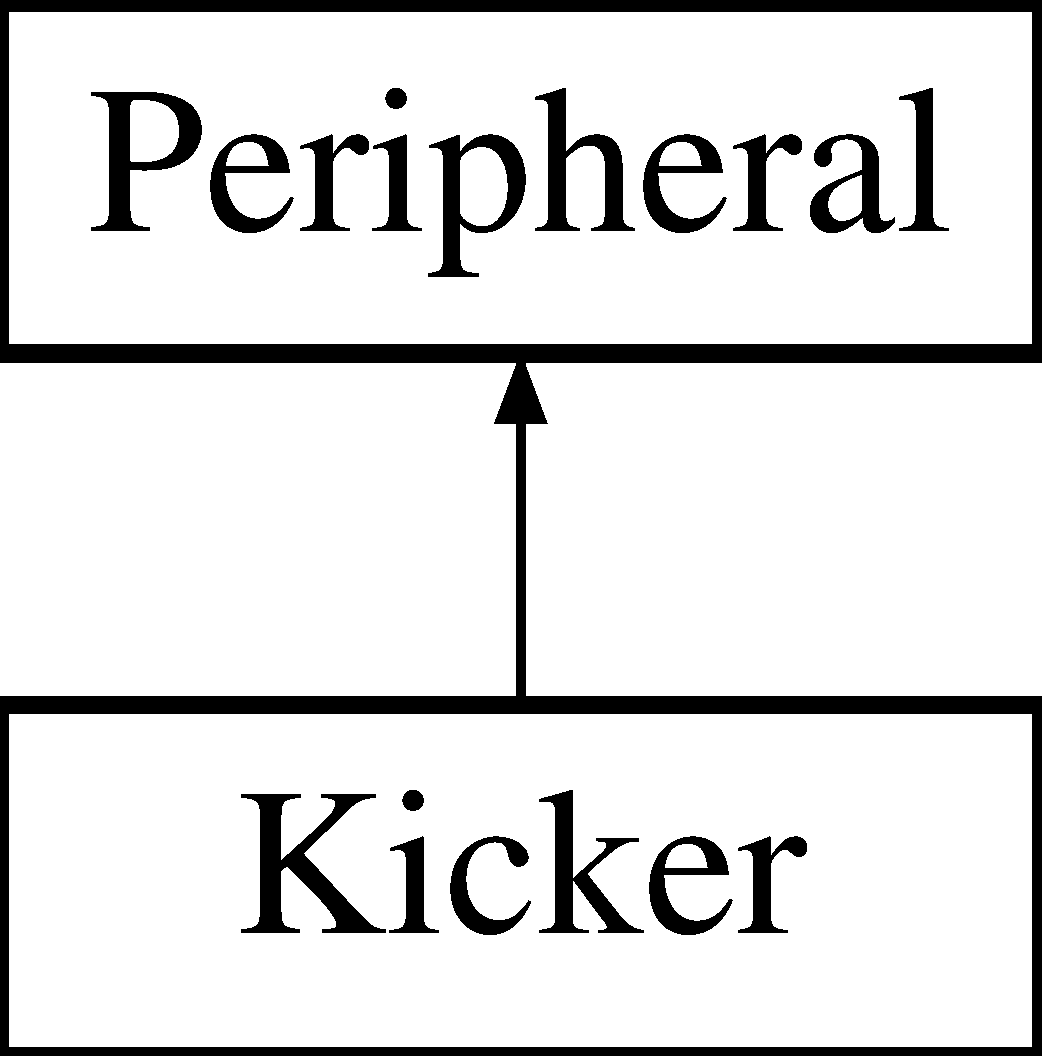
\includegraphics[height=2.000000cm]{class_kicker}
\end{center}
\end{figure}
\subsection*{Public Member Functions}
\begin{DoxyCompactItemize}
\item 
\mbox{\Hypertarget{class_kicker_a5cc008a16602853464a0db97672e7f7f}\label{class_kicker_a5cc008a16602853464a0db97672e7f7f}} 
void \mbox{\hyperlink{class_kicker_a5cc008a16602853464a0db97672e7f7f}{do\+Not\+Connected\+Thing}} ()
\begin{DoxyCompactList}\small\item\em ensure the robot enters a safe state when connection to the controller is lost \end{DoxyCompactList}\item 
\mbox{\Hypertarget{class_kicker_a21e66856229e39fa6a0872f25ecb850b}\label{class_kicker_a21e66856229e39fa6a0872f25ecb850b}} 
void \mbox{\hyperlink{class_kicker_a21e66856229e39fa6a0872f25ecb850b}{do\+Thing}} ()
\begin{DoxyCompactList}\small\item\em the implementation of do\+Thing should implement what happens when the controller is connected \end{DoxyCompactList}\item 
\mbox{\Hypertarget{class_kicker_a3b5caef78a0b6f07a37978763d42b131}\label{class_kicker_a3b5caef78a0b6f07a37978763d42b131}} 
void \mbox{\hyperlink{class_kicker_a3b5caef78a0b6f07a37978763d42b131}{setup}} ()
\begin{DoxyCompactList}\small\item\em sets initial values of variables \end{DoxyCompactList}\end{DoxyCompactItemize}


\subsection{Detailed Description}
This class controls the kicker peripheral. 

\begin{DoxyAuthor}{Author}
Bill Sullivan
\end{DoxyAuthor}
\begin{DoxyVersion}{Version}
\$\+Revision\+: 1.\+0
\end{DoxyVersion}
\begin{DoxyDate}{Date}
2018/08/15 14\+:16\+:20
\end{DoxyDate}
Created on\+: 2018/04/14 14\+:16\+:20 

The documentation for this class was generated from the following files\+:\begin{DoxyCompactItemize}
\item 
Robotic\+Football\+Peripherals/\+Kicker\+Foot/kicker.\+hpp\item 
Robotic\+Football\+Peripherals/\+Kicker\+Foot/kicker.\+cpp\end{DoxyCompactItemize}

\hypertarget{class_l_e_d}{}\section{L\+ED Class Reference}
\label{class_l_e_d}\index{L\+ED@{L\+ED}}


This class controls the robots L\+E\+Ds.  




{\ttfamily \#include $<$L\+E\+D.\+hpp$>$}

\subsection*{Public Member Functions}
\begin{DoxyCompactItemize}
\item 
\mbox{\Hypertarget{class_l_e_d_abb089672733ef180aa8cddc8d3a37d9e}\label{class_l_e_d_abb089672733ef180aa8cddc8d3a37d9e}} 
void \mbox{\hyperlink{class_l_e_d_abb089672733ef180aa8cddc8d3a37d9e}{setup}} ()
\begin{DoxyCompactList}\small\item\em sets initial values of variables \end{DoxyCompactList}\item 
void \mbox{\hyperlink{class_l_e_d_ad122ee4ef58452558498c249fc293870}{set\+Color}} (char color)
\begin{DoxyCompactList}\small\item\em sets the color of the \mbox{\hyperlink{class_l_e_d}{L\+ED}} \end{DoxyCompactList}\item 
\mbox{\Hypertarget{class_l_e_d_aaff2c983e84d429526ed087653bab10c}\label{class_l_e_d_aaff2c983e84d429526ed087653bab10c}} 
void \mbox{\hyperlink{class_l_e_d_aaff2c983e84d429526ed087653bab10c}{flash\+Led}} ()
\begin{DoxyCompactList}\small\item\em flash the leds in a perticular pattern ~\newline
pattern usually runs once when the microcontroller turns on Used to determine if leds are working \end{DoxyCompactList}\end{DoxyCompactItemize}
\subsection*{Public Attributes}
\begin{DoxyCompactItemize}
\item 
\mbox{\Hypertarget{class_l_e_d_abdf064808bc54c7ca18456de4f0df0a0}\label{class_l_e_d_abdf064808bc54c7ca18456de4f0df0a0}} 
char \mbox{\hyperlink{class_l_e_d_abdf064808bc54c7ca18456de4f0df0a0}{tackled\+Color}}
\begin{DoxyCompactList}\small\item\em color the robot should be when tackled \end{DoxyCompactList}\item 
\mbox{\Hypertarget{class_l_e_d_acea9ddf3407c6535463a509d04ddfeda}\label{class_l_e_d_acea9ddf3407c6535463a509d04ddfeda}} 
char \mbox{\hyperlink{class_l_e_d_acea9ddf3407c6535463a509d04ddfeda}{not\+Tackeled\+Color}}
\begin{DoxyCompactList}\small\item\em color the robot should be when not tackled \end{DoxyCompactList}\end{DoxyCompactItemize}


\subsection{Detailed Description}
This class controls the robots L\+E\+Ds. 

\begin{DoxyAuthor}{Author}
Bill Sullivan
\end{DoxyAuthor}
\begin{DoxyVersion}{Version}
\$\+Revision\+: 1.\+0
\end{DoxyVersion}
\begin{DoxyDate}{Date}
2018/08/15 14\+:16\+:20
\end{DoxyDate}
Created on\+: 2018/04/14 14\+:16\+:20 

\subsection{Member Function Documentation}
\mbox{\Hypertarget{class_l_e_d_ad122ee4ef58452558498c249fc293870}\label{class_l_e_d_ad122ee4ef58452558498c249fc293870}} 
\index{L\+ED@{L\+ED}!set\+Color@{set\+Color}}
\index{set\+Color@{set\+Color}!L\+ED@{L\+ED}}
\subsubsection{\texorpdfstring{set\+Color()}{setColor()}}
{\footnotesize\ttfamily void L\+E\+D\+::set\+Color (\begin{DoxyParamCaption}\item[{char}]{color }\end{DoxyParamCaption})}



sets the color of the \mbox{\hyperlink{class_l_e_d}{L\+ED}} 


\begin{DoxyParams}[1]{Parameters}
\mbox{\tt in}  & {\em color} & The color the \mbox{\hyperlink{class_l_e_d}{L\+ED}} should be R\+ED = \textquotesingle{}r\textquotesingle{} B\+L\+UE = \textquotesingle{}b\textquotesingle{} G\+R\+E\+EN = \textquotesingle{}g\textquotesingle{} \\
\hline
\end{DoxyParams}


The documentation for this class was generated from the following files\+:\begin{DoxyCompactItemize}
\item 
Robotic\+Football\+Peripherals/\+L\+E\+D/L\+E\+D.\+hpp\item 
Robotic\+Football\+Peripherals/\+L\+E\+D/L\+E\+D.\+cpp\end{DoxyCompactItemize}

\hypertarget{class_omni_drive_conrtoller}{}\section{Omni\+Drive\+Conrtoller Class Reference}
\label{class_omni_drive_conrtoller}\index{Omni\+Drive\+Conrtoller@{Omni\+Drive\+Conrtoller}}


This is the drive train for omniwheel robots Used for most four motor robots.  




{\ttfamily \#include $<$Omni\+Drive.\+hpp$>$}

Inheritance diagram for Omni\+Drive\+Conrtoller\+:\begin{figure}[H]
\begin{center}
\leavevmode
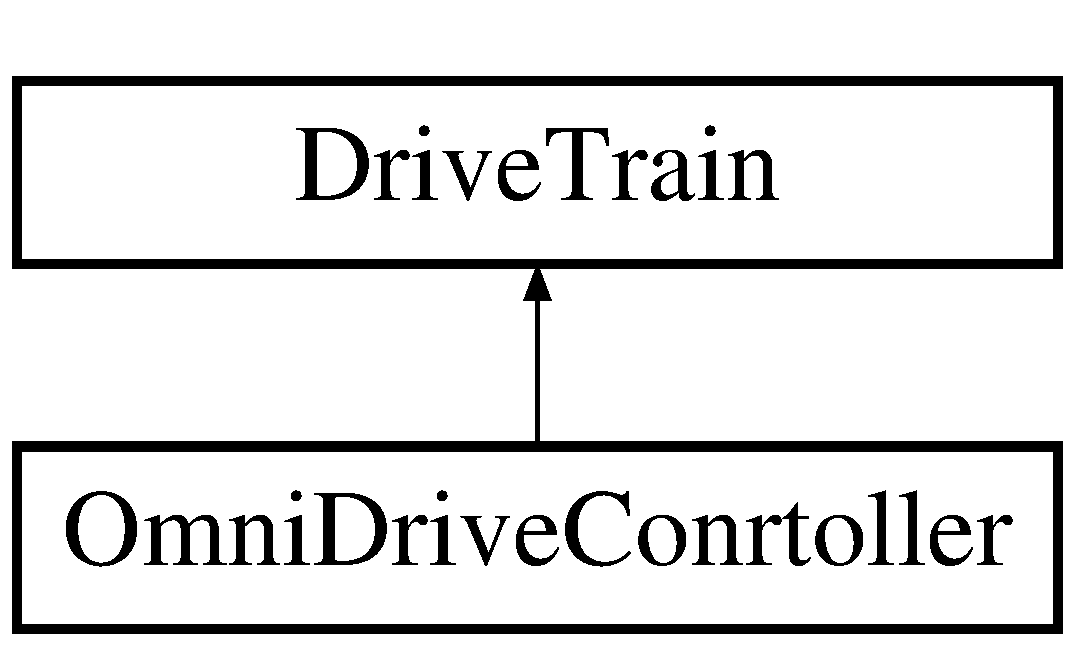
\includegraphics[height=2.000000cm]{class_omni_drive_conrtoller}
\end{center}
\end{figure}
\subsection*{Public Member Functions}
\begin{DoxyCompactItemize}
\item 
\mbox{\Hypertarget{class_omni_drive_conrtoller_afa3633aa507f94725e2708e64812fc0d}\label{class_omni_drive_conrtoller_afa3633aa507f94725e2708e64812fc0d}} 
void \mbox{\hyperlink{class_omni_drive_conrtoller_afa3633aa507f94725e2708e64812fc0d}{e\+Stop}} ()
\begin{DoxyCompactList}\small\item\em stop the robot so in the event control is lost controls what happens when the controller disconnects Make sure this code results in the robot stopping or we will break anouther door \end{DoxyCompactList}\item 
\mbox{\Hypertarget{class_omni_drive_conrtoller_a49df2da45a491575eaeed3ed08e6c06b}\label{class_omni_drive_conrtoller_a49df2da45a491575eaeed3ed08e6c06b}} 
void \mbox{\hyperlink{class_omni_drive_conrtoller_a49df2da45a491575eaeed3ed08e6c06b}{do\+Thing}} ()
\begin{DoxyCompactList}\small\item\em the implementation of do\+Thing should implement what happens when the controller is connected \end{DoxyCompactList}\item 
\mbox{\Hypertarget{class_omni_drive_conrtoller_a5cc239719ab846de89fbb9709f7a65c2}\label{class_omni_drive_conrtoller_a5cc239719ab846de89fbb9709f7a65c2}} 
void \mbox{\hyperlink{class_omni_drive_conrtoller_a5cc239719ab846de89fbb9709f7a65c2}{setup}} ()
\begin{DoxyCompactList}\small\item\em sets initial values of variables and motors \end{DoxyCompactList}\end{DoxyCompactItemize}
\subsection*{Protected Member Functions}
\begin{DoxyCompactItemize}
\item 
\mbox{\Hypertarget{class_omni_drive_conrtoller_a57c810f822a2fe5f49edad9ade0fb3eb}\label{class_omni_drive_conrtoller_a57c810f822a2fe5f49edad9ade0fb3eb}} 
void \mbox{\hyperlink{class_omni_drive_conrtoller_a57c810f822a2fe5f49edad9ade0fb3eb}{drive}} ()
\begin{DoxyCompactList}\small\item\em function that controls the robot \end{DoxyCompactList}\end{DoxyCompactItemize}
\subsection*{Protected Attributes}
\begin{DoxyCompactItemize}
\item 
\mbox{\Hypertarget{class_omni_drive_conrtoller_a0a78c1214005e227761e651657e66200}\label{class_omni_drive_conrtoller_a0a78c1214005e227761e651657e66200}} 
int \mbox{\hyperlink{class_omni_drive_conrtoller_a0a78c1214005e227761e651657e66200}{motor\+Correct}}
\begin{DoxyCompactList}\small\item\em variable that corrects for diffrences between each motor (Mostly irrlevent since bainbots moters were replaced) \end{DoxyCompactList}\item 
\mbox{\Hypertarget{class_omni_drive_conrtoller_af911b890cd2e146b211c0e7c4b53fc86}\label{class_omni_drive_conrtoller_af911b890cd2e146b211c0e7c4b53fc86}} 
int8\+\_\+t \mbox{\hyperlink{class_omni_drive_conrtoller_af911b890cd2e146b211c0e7c4b53fc86}{inverting}}
\begin{DoxyCompactList}\small\item\em variable that selects if robot is driving backwords \end{DoxyCompactList}\item 
\mbox{\Hypertarget{class_omni_drive_conrtoller_a03baba5698664886fece7c2bc1acd81b}\label{class_omni_drive_conrtoller_a03baba5698664886fece7c2bc1acd81b}} 
float {\bfseries motor\+Reverse}
\item 
\mbox{\Hypertarget{class_omni_drive_conrtoller_ac06677eaf663dafb06fec88cc7ca36a3}\label{class_omni_drive_conrtoller_ac06677eaf663dafb06fec88cc7ca36a3}} 
int8 int \mbox{\hyperlink{class_omni_drive_conrtoller_ac06677eaf663dafb06fec88cc7ca36a3}{turn\+Handicap}}
\begin{DoxyCompactList}\small\item\em motor power is divided by this variable for rotational motion \end{DoxyCompactList}\item 
\mbox{\Hypertarget{class_omni_drive_conrtoller_af9a59405abbb827a1ab9934561c0004d}\label{class_omni_drive_conrtoller_af9a59405abbb827a1ab9934561c0004d}} 
int8\+\_\+t \mbox{\hyperlink{class_omni_drive_conrtoller_af9a59405abbb827a1ab9934561c0004d}{handicap}}
\begin{DoxyCompactList}\small\item\em motor power is divided by this variable for linear motion \end{DoxyCompactList}\item 
\mbox{\Hypertarget{class_omni_drive_conrtoller_a8386f67e9931ac191335c14c4b56bbda}\label{class_omni_drive_conrtoller_a8386f67e9931ac191335c14c4b56bbda}} 
Servo \mbox{\hyperlink{class_omni_drive_conrtoller_a8386f67e9931ac191335c14c4b56bbda}{motor1}}
\begin{DoxyCompactList}\small\item\em Victors are modeled as servos. \end{DoxyCompactList}\item 
\mbox{\Hypertarget{class_omni_drive_conrtoller_aa4a56af43aad703ade2854b5a544c570}\label{class_omni_drive_conrtoller_aa4a56af43aad703ade2854b5a544c570}} 
Servo {\bfseries motor2}
\item 
\mbox{\Hypertarget{class_omni_drive_conrtoller_a28f94aa752f0fd8cd7de271d68c8cfe1}\label{class_omni_drive_conrtoller_a28f94aa752f0fd8cd7de271d68c8cfe1}} 
Servo {\bfseries motor3}
\item 
\mbox{\Hypertarget{class_omni_drive_conrtoller_a80bdd6e6a723aa9e101f738b6c35462f}\label{class_omni_drive_conrtoller_a80bdd6e6a723aa9e101f738b6c35462f}} 
Servo {\bfseries motor4}
\end{DoxyCompactItemize}


\subsection{Detailed Description}
This is the drive train for omniwheel robots Used for most four motor robots. 

\begin{DoxyAuthor}{Author}
Bill Sullivan
\end{DoxyAuthor}
\begin{DoxyVersion}{Version}
\$\+Revision\+: 1.\+0
\end{DoxyVersion}
\begin{DoxyDate}{Date}
2018/08/15 14\+:16\+:20
\end{DoxyDate}
Created on\+: 2018/04/14 14\+:16\+:20 

The documentation for this class was generated from the following files\+:\begin{DoxyCompactItemize}
\item 
Drive\+Train/\+Omni\+Drive/Omni\+Drive.\+hpp\item 
Drive\+Train/\+Omni\+Drive/Omni\+Drive.\+cpp\end{DoxyCompactItemize}

\hypertarget{classomni_drive_conrtoller}{}\section{omni\+Drive\+Conrtoller Class Reference}
\label{classomni_drive_conrtoller}\index{omni\+Drive\+Conrtoller@{omni\+Drive\+Conrtoller}}


The documentation for this class was generated from the following file\+:\begin{DoxyCompactItemize}
\item 
Drive\+Train/\+Omni\+Drive/\+Rotation\+Lock/Rotation\+Lock\+Omni\+Drive.\+hpp\end{DoxyCompactItemize}

\hypertarget{class_peripheral}{}\section{Peripheral Class Reference}
\label{class_peripheral}\index{Peripheral@{Peripheral}}


This class is the parent class for all other drive trains.  




{\ttfamily \#include $<$Peripheral.\+hpp$>$}

Inheritance diagram for Peripheral\+:\begin{figure}[H]
\begin{center}
\leavevmode
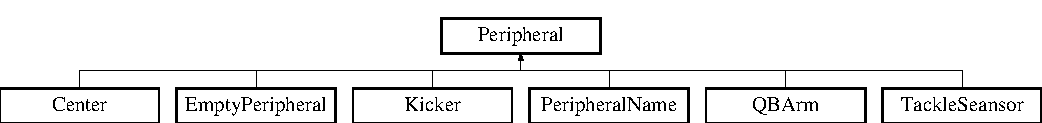
\includegraphics[height=1.651917cm]{class_peripheral}
\end{center}
\end{figure}
\subsection*{Public Member Functions}
\begin{DoxyCompactItemize}
\item 
\mbox{\Hypertarget{class_peripheral_adc231eaa2fec43878c139af159503727}\label{class_peripheral_adc231eaa2fec43878c139af159503727}} 
void \mbox{\hyperlink{class_peripheral_adc231eaa2fec43878c139af159503727}{do\+Not\+Connected\+Thing}} ()
\begin{DoxyCompactList}\small\item\em ensure the robot enters a safe state when connection to the controller is lost \end{DoxyCompactList}\item 
\mbox{\Hypertarget{class_peripheral_a5baf1180b80d1a61192542c29ae1d650}\label{class_peripheral_a5baf1180b80d1a61192542c29ae1d650}} 
void \mbox{\hyperlink{class_peripheral_a5baf1180b80d1a61192542c29ae1d650}{do\+Thing}} ()
\begin{DoxyCompactList}\small\item\em the implementation of do\+Thing should implement what happens when the controller is connected \end{DoxyCompactList}\item 
\mbox{\Hypertarget{class_peripheral_a3571b35c82ab213985cb1693be08904b}\label{class_peripheral_a3571b35c82ab213985cb1693be08904b}} 
void \mbox{\hyperlink{class_peripheral_a3571b35c82ab213985cb1693be08904b}{setup}} ()
\begin{DoxyCompactList}\small\item\em sets initial values of variables \end{DoxyCompactList}\end{DoxyCompactItemize}


\subsection{Detailed Description}
This class is the parent class for all other drive trains. 

This class is the parent class for all other drive trains

The only way this class should be used is as a parent class for other classes

\begin{DoxyAuthor}{Author}
Bill Sullivan
\end{DoxyAuthor}
\begin{DoxyVersion}{Version}
\$\+Revision\+: 1.\+0
\end{DoxyVersion}
\begin{DoxyDate}{Date}
2018/08/15 14\+:16\+:20
\end{DoxyDate}
Created on\+: 2018/04/14 14\+:16\+:20 

The documentation for this class was generated from the following file\+:\begin{DoxyCompactItemize}
\item 
Peripheral.\+hpp\end{DoxyCompactItemize}

\hypertarget{class_peripheral_name}{}\section{Peripheral\+Name Class Reference}
\label{class_peripheral_name}\index{Peripheral\+Name@{Peripheral\+Name}}


Provide an example.  




{\ttfamily \#include $<$Example\+Peripheral.\+hpp$>$}

Inheritance diagram for Peripheral\+Name\+:\begin{figure}[H]
\begin{center}
\leavevmode
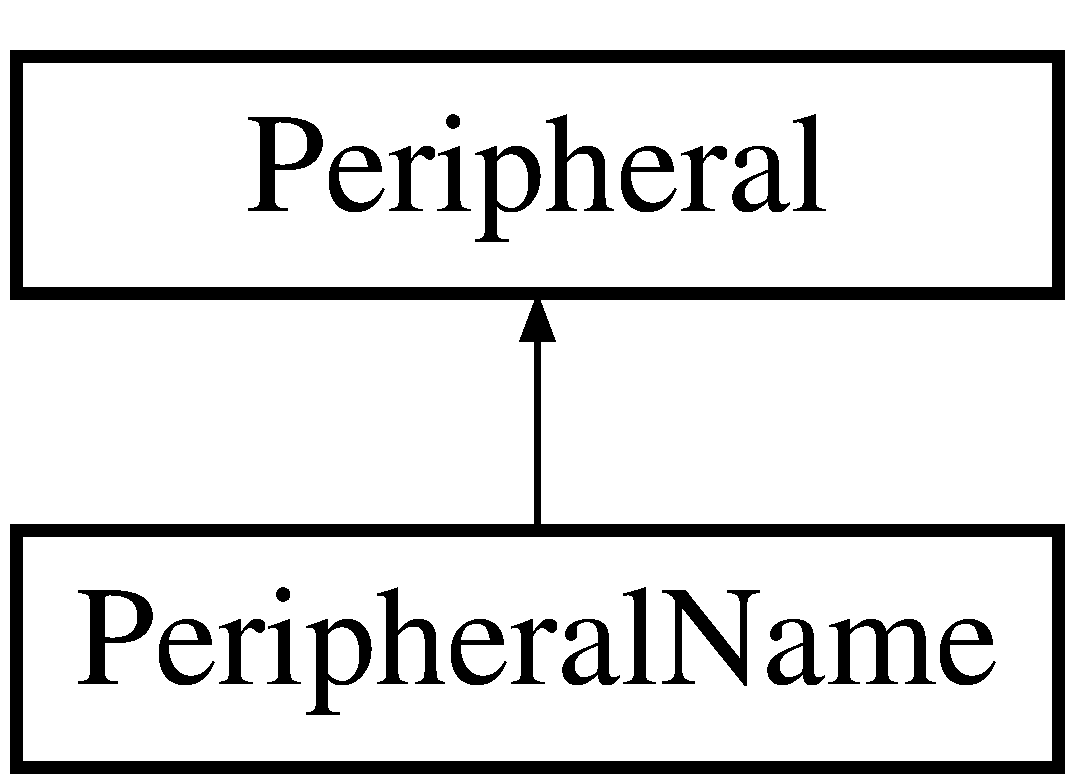
\includegraphics[height=2.000000cm]{class_peripheral_name}
\end{center}
\end{figure}
\subsection*{Public Member Functions}
\begin{DoxyCompactItemize}
\item 
void \mbox{\hyperlink{class_peripheral_name_a42388889799a14fd6cda2c2819b0e38d}{do\+Thing}} ()
\begin{DoxyCompactList}\small\item\em Function that runs every loop when controller is connected. \end{DoxyCompactList}\item 
void \mbox{\hyperlink{class_peripheral_name_a63b193d5328d4800de3bb8905f1d2f20}{do\+Not\+Connected\+Thing}} ()
\begin{DoxyCompactList}\small\item\em Function that runs every loop when controller is not connected. \end{DoxyCompactList}\item 
void \mbox{\hyperlink{class_peripheral_name_aa6b1719095b6e25d80a2567f400316db}{setup}} ()
\begin{DoxyCompactList}\small\item\em Function that runs once when the microcontroller turns on. \end{DoxyCompactList}\end{DoxyCompactItemize}


\subsection{Detailed Description}
Provide an example. 

This class is meant as an example. It is not useful by itself rather its usefulness is only a function of how much it helps the reader. It is in a sense defined by the person who reads it and otherwise does not exist in any real form.

\begin{DoxyNote}{Note}
Attempts at zen rarely work.
\end{DoxyNote}
\begin{DoxyAuthor}{Author}
Bill Sullivan
\end{DoxyAuthor}
\begin{DoxyVersion}{Version}
\$\+Revision\+: 1.\+0
\end{DoxyVersion}
\begin{DoxyDate}{Date}
2018/08/14 14\+:16\+:20
\end{DoxyDate}
Created on\+: 2018/04/14 14\+:16\+:20

\begin{DoxyParagraph}{Id}
doxygen-\/howto2.\+html,v 1.\+5 bv Exp 
\end{DoxyParagraph}


\subsection{Member Function Documentation}
\mbox{\Hypertarget{class_peripheral_name_a63b193d5328d4800de3bb8905f1d2f20}\label{class_peripheral_name_a63b193d5328d4800de3bb8905f1d2f20}} 
\index{Peripheral\+Name@{Peripheral\+Name}!do\+Not\+Connected\+Thing@{do\+Not\+Connected\+Thing}}
\index{do\+Not\+Connected\+Thing@{do\+Not\+Connected\+Thing}!Peripheral\+Name@{Peripheral\+Name}}
\subsubsection{\texorpdfstring{do\+Not\+Connected\+Thing()}{doNotConnectedThing()}}
{\footnotesize\ttfamily void Peripheral\+Name\+::do\+Not\+Connected\+Thing (\begin{DoxyParamCaption}{ }\end{DoxyParamCaption})\hspace{0.3cm}{\ttfamily [inline]}}



Function that runs every loop when controller is not connected. 

Function that runs every loop when controller not is connected. Fill in more relevent comments here in your peripheral implementation \mbox{\Hypertarget{class_peripheral_name_a42388889799a14fd6cda2c2819b0e38d}\label{class_peripheral_name_a42388889799a14fd6cda2c2819b0e38d}} 
\index{Peripheral\+Name@{Peripheral\+Name}!do\+Thing@{do\+Thing}}
\index{do\+Thing@{do\+Thing}!Peripheral\+Name@{Peripheral\+Name}}
\subsubsection{\texorpdfstring{do\+Thing()}{doThing()}}
{\footnotesize\ttfamily void Peripheral\+Name\+::do\+Thing (\begin{DoxyParamCaption}{ }\end{DoxyParamCaption})\hspace{0.3cm}{\ttfamily [inline]}}



Function that runs every loop when controller is connected. 

Function that runs every loop when controller is connected. Fill in more relevent comments here in your peripheral implementation \mbox{\Hypertarget{class_peripheral_name_aa6b1719095b6e25d80a2567f400316db}\label{class_peripheral_name_aa6b1719095b6e25d80a2567f400316db}} 
\index{Peripheral\+Name@{Peripheral\+Name}!setup@{setup}}
\index{setup@{setup}!Peripheral\+Name@{Peripheral\+Name}}
\subsubsection{\texorpdfstring{setup()}{setup()}}
{\footnotesize\ttfamily void Peripheral\+Name\+::setup (\begin{DoxyParamCaption}{ }\end{DoxyParamCaption})\hspace{0.3cm}{\ttfamily [inline]}}



Function that runs once when the microcontroller turns on. 

Function that runs once when the microcontroller turns on. Fill in more relevent comments here in your peripheral implementation 

The documentation for this class was generated from the following file\+:\begin{DoxyCompactItemize}
\item 
Robotic\+Football\+Peripherals/\+Example\+Peripheral/Example\+Peripheral.\+hpp\end{DoxyCompactItemize}

\hypertarget{class_q_b_arm}{}\section{Q\+B\+Arm Class Reference}
\label{class_q_b_arm}\index{Q\+B\+Arm@{Q\+B\+Arm}}


This class controls the quaterback\textquotesingle{}s arm.  




{\ttfamily \#include $<$Q\+B\+Arm.\+hpp$>$}

Inheritance diagram for Q\+B\+Arm\+:\begin{figure}[H]
\begin{center}
\leavevmode
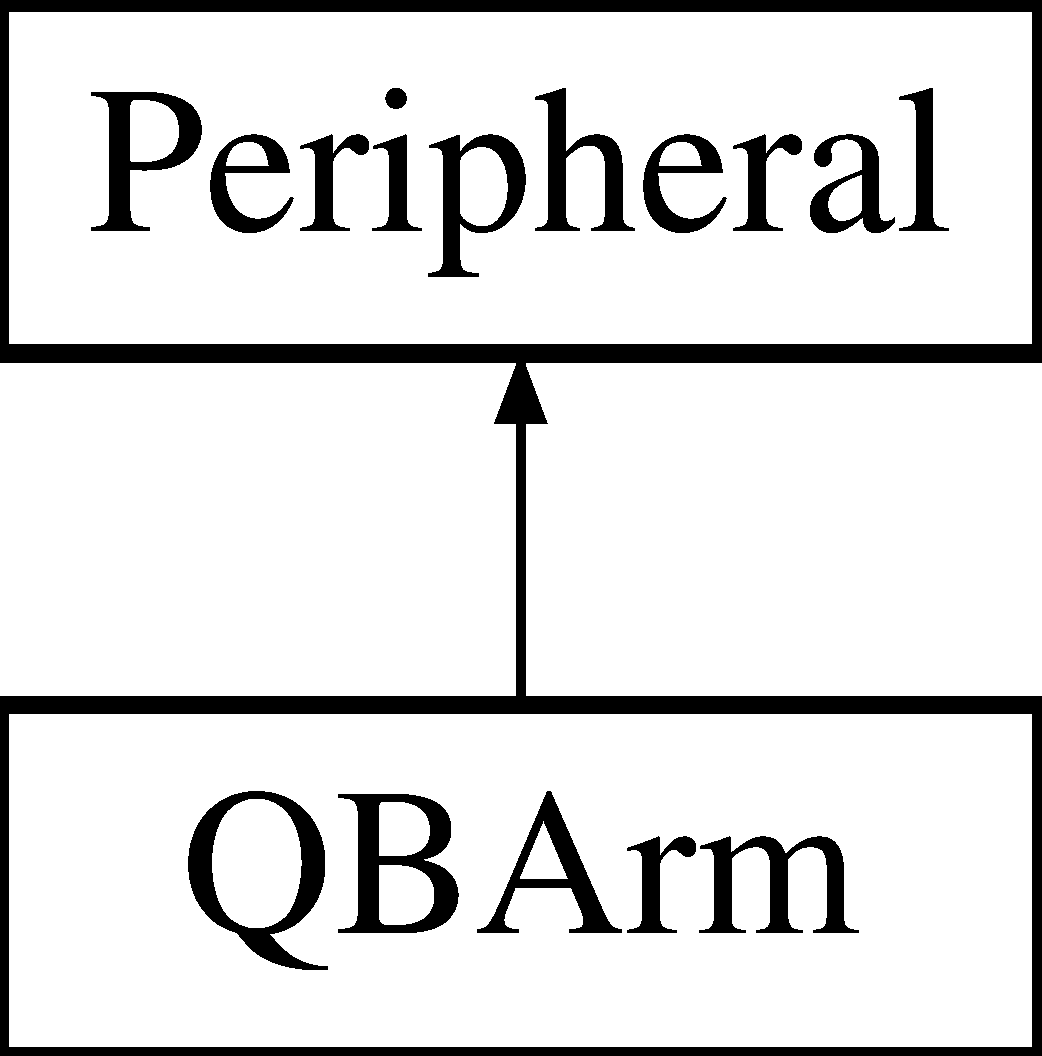
\includegraphics[height=2.000000cm]{class_q_b_arm}
\end{center}
\end{figure}
\subsection*{Public Member Functions}
\begin{DoxyCompactItemize}
\item 
\mbox{\Hypertarget{class_q_b_arm_aa9f699ba82995b84b6b48361d83c3e4f}\label{class_q_b_arm_aa9f699ba82995b84b6b48361d83c3e4f}} 
void \mbox{\hyperlink{class_q_b_arm_aa9f699ba82995b84b6b48361d83c3e4f}{do\+Not\+Connected\+Thing}} ()
\begin{DoxyCompactList}\small\item\em ensure the robot enters a safe state when connection to the controller is lost \end{DoxyCompactList}\item 
\mbox{\Hypertarget{class_q_b_arm_af1729cc1a588e5d996677bccb6b09237}\label{class_q_b_arm_af1729cc1a588e5d996677bccb6b09237}} 
void \mbox{\hyperlink{class_q_b_arm_af1729cc1a588e5d996677bccb6b09237}{do\+Thing}} ()
\begin{DoxyCompactList}\small\item\em the implementation of do\+Thing should implement what happens when the controller is connected \end{DoxyCompactList}\item 
\mbox{\Hypertarget{class_q_b_arm_abfef9dc751d9e484f480571aeb875a37}\label{class_q_b_arm_abfef9dc751d9e484f480571aeb875a37}} 
void \mbox{\hyperlink{class_q_b_arm_abfef9dc751d9e484f480571aeb875a37}{setup}} ()
\begin{DoxyCompactList}\small\item\em sets initial values of variables \end{DoxyCompactList}\end{DoxyCompactItemize}


\subsection{Detailed Description}
This class controls the quaterback\textquotesingle{}s arm. 

\begin{DoxyAuthor}{Author}
Bill Sullivan
\end{DoxyAuthor}
\begin{DoxyVersion}{Version}
\$\+Revision\+: 1.\+0
\end{DoxyVersion}
\begin{DoxyDate}{Date}
2018/08/15 14\+:16\+:20
\end{DoxyDate}
Created on\+: 2018/04/14 14\+:16\+:20 

The documentation for this class was generated from the following files\+:\begin{DoxyCompactItemize}
\item 
Robotic\+Football\+Peripherals/\+Q\+B\+Arm/Q\+B\+Arm.\+hpp\item 
Robotic\+Football\+Peripherals/\+Q\+B\+Arm/Q\+B\+Arm.\+cpp\end{DoxyCompactItemize}

\hypertarget{class_robot}{}\section{Robot Class Reference}
\label{class_robot}\index{Robot@{Robot}}


Class that acts as a wrapper for other classes.  




{\ttfamily \#include $<$Robot.\+hpp$>$}

\subsection*{Public Member Functions}
\begin{DoxyCompactItemize}
\item 
\mbox{\Hypertarget{class_robot_a1fc37e3c329d59795f6adf44199d4df9}\label{class_robot_a1fc37e3c329d59795f6adf44199d4df9}} 
void \mbox{\hyperlink{class_robot_a1fc37e3c329d59795f6adf44199d4df9}{setup}} ()
\begin{DoxyCompactList}\small\item\em Function that sets up the rest of the firmware setup function initilizes all variables sets up setial port to connect back to computer use to program the microcontroller. \end{DoxyCompactList}\item 
void \mbox{\hyperlink{class_robot_ad92e1e27045a02533f55ecab2b16d368}{loop}} ()
\begin{DoxyCompactList}\small\item\em Function that runs every to its end then repeats until device shutdown chekcs if controller is connectd if it is setup controller on first loop after connection then run drive train and peripheral\textquotesingle{}s connected code if it is not run drive train and peripheral\textquotesingle{}s not connected code. \end{DoxyCompactList}\end{DoxyCompactItemize}
\subsection*{Protected Member Functions}
\begin{DoxyCompactItemize}
\item 
void \mbox{\hyperlink{class_robot_aca73cd3e3582f49cc0b33ee900cbc245}{new\+Connection}} ()
\begin{DoxyCompactList}\small\item\em Function that runs when P\+S3 Controller connects. \end{DoxyCompactList}\end{DoxyCompactItemize}
\subsection*{Protected Attributes}
\begin{DoxyCompactItemize}
\item 
\mbox{\hyperlink{class_drive_train}{Drive\+Train}} $\ast$ \mbox{\hyperlink{class_robot_a4b499841182a38720a26a493fa98363a}{drive\+Train}}
\begin{DoxyCompactList}\small\item\em Pointer to an \mbox{\hyperlink{class_l_e_d}{L\+ED}}. \end{DoxyCompactList}\item 
\mbox{\hyperlink{class_valpo_robotics_1_1array}{Valpo\+Robotics\+::array}}$<$ \mbox{\hyperlink{class_peripheral}{Peripheral}} $\ast$, M\+A\+X\+\_\+\+T\+O\+T\+A\+L\+\_\+\+P\+E\+R\+I\+P\+E\+R\+A\+LS $>$ \mbox{\hyperlink{class_robot_a8db438771a3e7dc9d2cf5dd2e1d25f74}{peripheral\+Vec}}
\begin{DoxyCompactList}\small\item\em Array of pointers to Peripherals. \end{DoxyCompactList}\item 
\mbox{\Hypertarget{class_robot_a19c7a18705cf4bc4359f5ba12c3541d8}\label{class_robot_a19c7a18705cf4bc4359f5ba12c3541d8}} 
bool \mbox{\hyperlink{class_robot_a19c7a18705cf4bc4359f5ba12c3541d8}{newconnect}}
\begin{DoxyCompactList}\small\item\em variable that tracks if the controller is connected \end{DoxyCompactList}\end{DoxyCompactItemize}


\subsection{Detailed Description}
Class that acts as a wrapper for other classes. 

This class enables each peipheral and drivetrain to be run without having to know what the other peripherals are doing

\begin{DoxyNote}{Note}
Attempts at zen rarely work.
\end{DoxyNote}
\begin{DoxyAuthor}{Author}
Bill Sullivan
\end{DoxyAuthor}
\begin{DoxyVersion}{Version}
\$\+Revision\+: 1.\+0
\end{DoxyVersion}
\begin{DoxyDate}{Date}
2018/08/15 14\+:16\+:20
\end{DoxyDate}
Created on\+: 2018/04/14 14\+:16\+:20

\begin{DoxyParagraph}{Id}
doxygen-\/howto2.\+html,v 1.\+5 bv Exp 
\end{DoxyParagraph}


\subsection{Member Function Documentation}
\mbox{\Hypertarget{class_robot_ad92e1e27045a02533f55ecab2b16d368}\label{class_robot_ad92e1e27045a02533f55ecab2b16d368}} 
\index{Robot@{Robot}!loop@{loop}}
\index{loop@{loop}!Robot@{Robot}}
\subsubsection{\texorpdfstring{loop()}{loop()}}
{\footnotesize\ttfamily void Robot\+::loop (\begin{DoxyParamCaption}{ }\end{DoxyParamCaption})\hspace{0.3cm}{\ttfamily [inline]}}



Function that runs every to its end then repeats until device shutdown chekcs if controller is connectd if it is setup controller on first loop after connection then run drive train and peripheral\textquotesingle{}s connected code if it is not run drive train and peripheral\textquotesingle{}s not connected code. 

sets up setial port to connect back to computer use to program the microcontroller \mbox{\Hypertarget{class_robot_aca73cd3e3582f49cc0b33ee900cbc245}\label{class_robot_aca73cd3e3582f49cc0b33ee900cbc245}} 
\index{Robot@{Robot}!new\+Connection@{new\+Connection}}
\index{new\+Connection@{new\+Connection}!Robot@{Robot}}
\subsubsection{\texorpdfstring{new\+Connection()}{newConnection()}}
{\footnotesize\ttfamily void Robot\+::new\+Connection (\begin{DoxyParamCaption}{ }\end{DoxyParamCaption})\hspace{0.3cm}{\ttfamily [inline]}, {\ttfamily [protected]}}



Function that runs when P\+S3 Controller connects. 

Function that runs when P\+S3 Controller connects Function tells rest of the firmware and the user that the controller has connected 

\subsection{Member Data Documentation}
\mbox{\Hypertarget{class_robot_a4b499841182a38720a26a493fa98363a}\label{class_robot_a4b499841182a38720a26a493fa98363a}} 
\index{Robot@{Robot}!drive\+Train@{drive\+Train}}
\index{drive\+Train@{drive\+Train}!Robot@{Robot}}
\subsubsection{\texorpdfstring{drive\+Train}{driveTrain}}
{\footnotesize\ttfamily \mbox{\hyperlink{class_drive_train}{Drive\+Train}}$\ast$ Robot\+::drive\+Train\hspace{0.3cm}{\ttfamily [protected]}}



Pointer to an \mbox{\hyperlink{class_l_e_d}{L\+ED}}. 

Pointer to an \mbox{\hyperlink{class_l_e_d}{L\+ED}} Stores an pointer to an \mbox{\hyperlink{class_l_e_d}{L\+ED}} class so that all peipherals that acces the \mbox{\hyperlink{class_l_e_d}{L\+ED}} (ie the Tackle Sensor) access the same \mbox{\hyperlink{class_l_e_d}{L\+ED}} Pointer to a \mbox{\hyperlink{class_drive_train}{Drive\+Train}}

e\+Stop is run when the controller is disconnected do\+Thing runs continously when the controller is connected setup runs once when the microcontroller is turned on \mbox{\Hypertarget{class_robot_a8db438771a3e7dc9d2cf5dd2e1d25f74}\label{class_robot_a8db438771a3e7dc9d2cf5dd2e1d25f74}} 
\index{Robot@{Robot}!peripheral\+Vec@{peripheral\+Vec}}
\index{peripheral\+Vec@{peripheral\+Vec}!Robot@{Robot}}
\subsubsection{\texorpdfstring{peripheral\+Vec}{peripheralVec}}
{\footnotesize\ttfamily \mbox{\hyperlink{class_valpo_robotics_1_1array}{Valpo\+Robotics\+::array}}$<$\mbox{\hyperlink{class_peripheral}{Peripheral}}$\ast$, M\+A\+X\+\_\+\+T\+O\+T\+A\+L\+\_\+\+P\+E\+R\+I\+P\+E\+R\+A\+LS$>$ Robot\+::peripheral\+Vec\hspace{0.3cm}{\ttfamily [protected]}}



Array of pointers to Peripherals. 

do\+Not\+Connected\+Thing is run when the controller is disconnected do\+Thing runs continously when the controller is connected setup runs once when the microcontroller is turned on 

The documentation for this class was generated from the following file\+:\begin{DoxyCompactItemize}
\item 
Robot.\+hpp\end{DoxyCompactItemize}

\hypertarget{class_tackle_seansor}{}\section{Tackle\+Seansor Class Reference}
\label{class_tackle_seansor}\index{Tackle\+Seansor@{Tackle\+Seansor}}


This class controls the tackle sensor and its interaction with the L\+E\+Ds.  




{\ttfamily \#include $<$tackle.\+hpp$>$}

Inheritance diagram for Tackle\+Seansor\+:\begin{figure}[H]
\begin{center}
\leavevmode
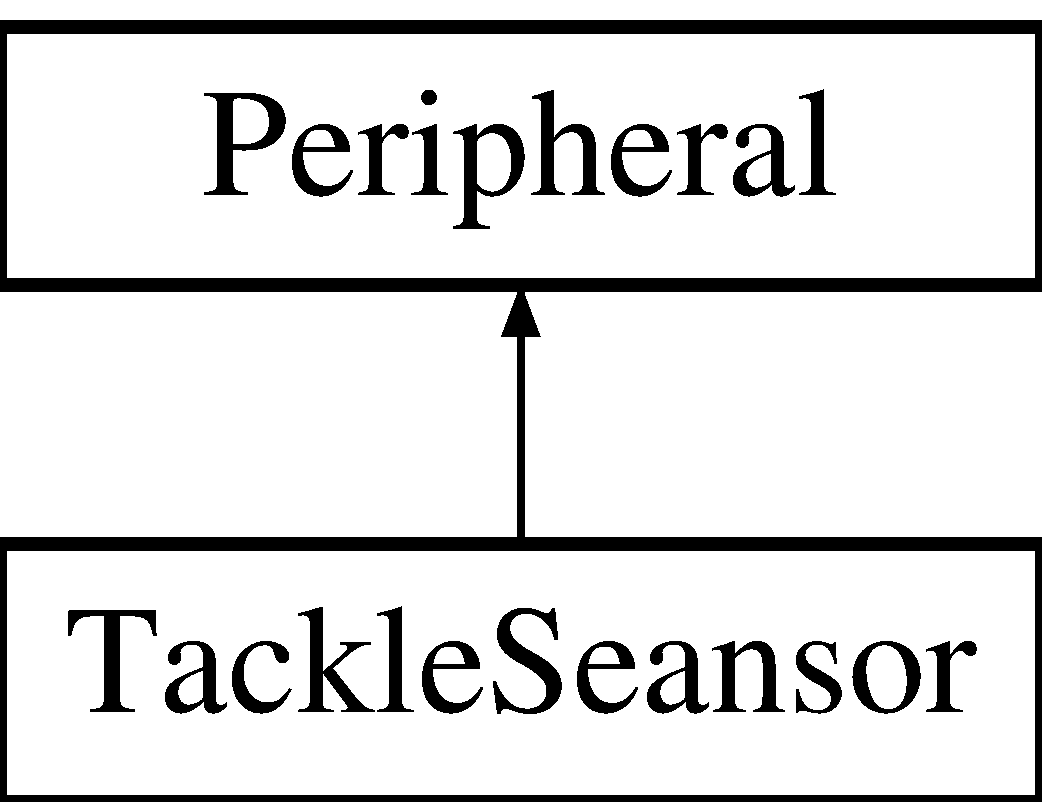
\includegraphics[height=2.000000cm]{class_tackle_seansor}
\end{center}
\end{figure}
\subsection*{Public Member Functions}
\begin{DoxyCompactItemize}
\item 
\mbox{\Hypertarget{class_tackle_seansor_ab545daa8fffd28ecf2c2210ecfeb5e7d}\label{class_tackle_seansor_ab545daa8fffd28ecf2c2210ecfeb5e7d}} 
void \mbox{\hyperlink{class_tackle_seansor_ab545daa8fffd28ecf2c2210ecfeb5e7d}{do\+Not\+Connected\+Thing}} ()
\begin{DoxyCompactList}\small\item\em ensure the robot enters a safe state when connection to the controller is lost \end{DoxyCompactList}\item 
\mbox{\Hypertarget{class_tackle_seansor_a11a7aaec039344fd04ae94cf50545d6c}\label{class_tackle_seansor_a11a7aaec039344fd04ae94cf50545d6c}} 
void \mbox{\hyperlink{class_tackle_seansor_a11a7aaec039344fd04ae94cf50545d6c}{do\+Thing}} ()
\begin{DoxyCompactList}\small\item\em the implementation of do\+Thing should implement what happens when the controller is connected \end{DoxyCompactList}\item 
\mbox{\Hypertarget{class_tackle_seansor_a36060a6a6e62d3e4077fa29c49724ddc}\label{class_tackle_seansor_a36060a6a6e62d3e4077fa29c49724ddc}} 
void \mbox{\hyperlink{class_tackle_seansor_a36060a6a6e62d3e4077fa29c49724ddc}{setup}} ()
\begin{DoxyCompactList}\small\item\em sets initial values of variables \end{DoxyCompactList}\item 
\mbox{\Hypertarget{class_tackle_seansor_af276afe841ebe04d7073cc802350cbec}\label{class_tackle_seansor_af276afe841ebe04d7073cc802350cbec}} 
\mbox{\hyperlink{class_tackle_seansor_af276afe841ebe04d7073cc802350cbec}{Tackle\+Seansor}} (\mbox{\hyperlink{class_l_e_d}{L\+ED}} $\ast$\+\_\+p\+L\+ED)
\begin{DoxyCompactList}\small\item\em initilizes pointer to \mbox{\hyperlink{class_l_e_d}{L\+ED}} \end{DoxyCompactList}\end{DoxyCompactItemize}


\subsection{Detailed Description}
This class controls the tackle sensor and its interaction with the L\+E\+Ds. 

\begin{DoxyAuthor}{Author}
Bill Sullivan
\end{DoxyAuthor}
\begin{DoxyVersion}{Version}
\$\+Revision\+: 1.\+0
\end{DoxyVersion}
\begin{DoxyDate}{Date}
2018/08/15 14\+:16\+:20
\end{DoxyDate}
Created on\+: 2018/04/14 14\+:16\+:20 

The documentation for this class was generated from the following files\+:\begin{DoxyCompactItemize}
\item 
Robotic\+Football\+Peripherals/\+Tackle\+Sensor/tackle.\+hpp\item 
Robotic\+Football\+Peripherals/\+Tackle\+Sensor/tackle.\+cpp\end{DoxyCompactItemize}

\hypertarget{classtest_drive_conrtoller}{}\section{test\+Drive\+Conrtoller Class Reference}
\label{classtest_drive_conrtoller}\index{test\+Drive\+Conrtoller@{test\+Drive\+Conrtoller}}
Inheritance diagram for test\+Drive\+Conrtoller\+:\begin{figure}[H]
\begin{center}
\leavevmode
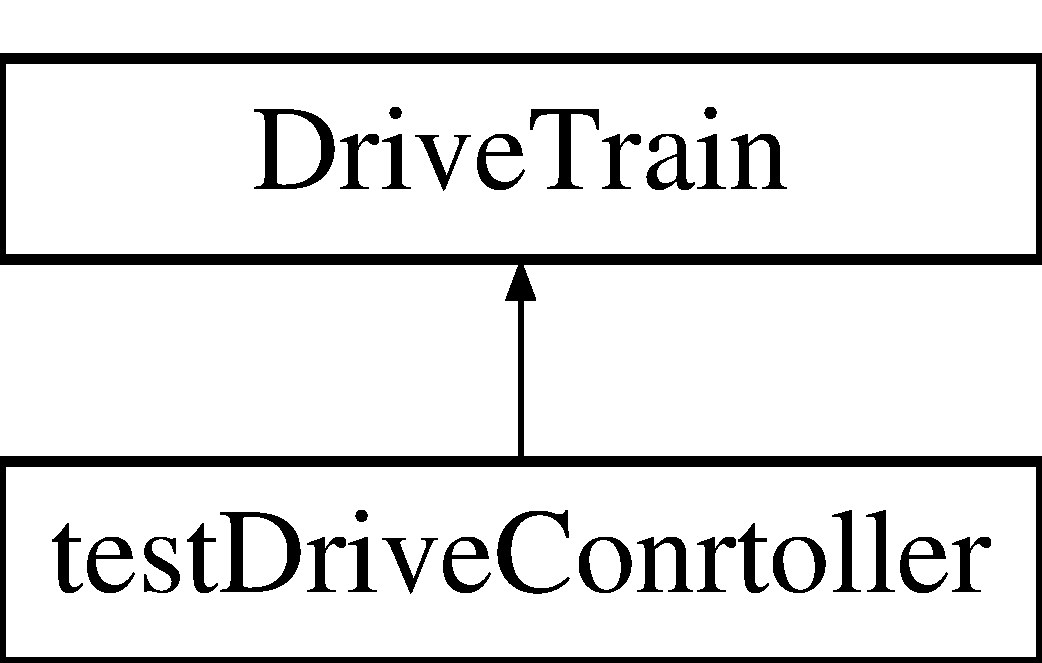
\includegraphics[height=2.000000cm]{classtest_drive_conrtoller}
\end{center}
\end{figure}
\subsection*{Public Member Functions}
\begin{DoxyCompactItemize}
\item 
\mbox{\Hypertarget{classtest_drive_conrtoller_ab2b6333c390e7b5f5988cf97c3fbaf0d}\label{classtest_drive_conrtoller_ab2b6333c390e7b5f5988cf97c3fbaf0d}} 
void \mbox{\hyperlink{classtest_drive_conrtoller_ab2b6333c390e7b5f5988cf97c3fbaf0d}{e\+Stop}} ()
\begin{DoxyCompactList}\small\item\em the implementation of e\+Stop should implement what happens when the controller disconnects Make sure this code results in the robot stopping or we will break anouther door \end{DoxyCompactList}\item 
\mbox{\Hypertarget{classtest_drive_conrtoller_ae093990e6c81832e1c5ba326c29dc1c8}\label{classtest_drive_conrtoller_ae093990e6c81832e1c5ba326c29dc1c8}} 
void \mbox{\hyperlink{classtest_drive_conrtoller_ae093990e6c81832e1c5ba326c29dc1c8}{do\+Thing}} ()
\begin{DoxyCompactList}\small\item\em the implementation of do\+Thing should implement what happens when the controller is connected \end{DoxyCompactList}\end{DoxyCompactItemize}


The documentation for this class was generated from the following file\+:\begin{DoxyCompactItemize}
\item 
Drive\+Train/\+Test\+Drive/Test\+Drive.\+hpp\end{DoxyCompactItemize}

%--- End generated contents ---

% Index
\backmatter
\newpage
\phantomsection
\clearemptydoublepage
\addcontentsline{toc}{chapter}{Index}
\printindex

\end{document}
